\documentclass[11pt]{article}

\usepackage{url}
\usepackage[font=footnotesize,labelfont=bf]{caption}
\usepackage{graphicx}
\usepackage[scientific-notation=true]{siunitx}
\usepackage{subcaption}
\usepackage{setspace}
\usepackage[top=0.6 in, bottom=0.7 in, left=0.7in, right=0.7in]{geometry}
\usepackage{blindtext}
\usepackage[utf8]{inputenc}
\usepackage{setspace}
\usepackage{vector}
\usepackage{amsmath}
\usepackage{empheq}
\usepackage{amssymb}
\usepackage{tgtermes}
\usepackage{gensymb}
\DeclareGraphicsExtensions{.pdf,.png,.jpg}
\usepackage{epstopdf}
\usepackage[singlelinecheck=false]{caption}
\usepackage[hyperfootnotes=false, pdfnewwindow, colorlinks=true]{hyperref}
\usepackage[title]{appendix}
\usepackage[section]{placeins}
\usepackage{float}

\AtBeginDocument{% optionally set colors to your liking
  \hypersetup{
    urlcolor=blue,
    citecolor=blue,
    linkcolor=blue,
  }%
}

\begin{document}



\title{\Large \bf{Optics Optimization for the D(e,e'p)n Experiment (E12-10-003)}}

\author{Carlos Yero}

\date{\today}
\maketitle



%*****************************************************************************************************************************************************
\section{Introduction}
\noindent The commissioning of the HMS/SHMS optics took place on the 2017-18 run period and underwent multiple revisions of the reconstruction
matrix elements for both spectrometers during that period.\cite{HMS_Optics, SHMS_Optics} This document presents the optics optimization checks
and procedures done on the High Momentum Spectrometer (HMS) and superHMS (SHMS) for the Deuteron Electro-Disintegration Commissioning Experiment
(E12-10-003) on April 2018. At the time, this experiment also served as part of the general optics commissioning as during data-taking, it was found that
the SHMS Q3 magnet had an un-ncecessary correction in the matrix elements. As a result, the data for this experiment is divided into two sections.
Only the section after the fix in the SHMS optics was used in the optimization procedure.\\
\indent The problem of optics optimization can be approached in different ways, depending on the circumstances
of the experiment. In this particular experiment, a series of H(e,e'p) elastic runs were taken at different
configurations such as to cover the entire HMS momentum range in the D(e,e'p)n reaction kinematics. The original
and corrected H(e,e'p) kinematics are summarized below.

\begin{table}[ht]
\begin{tabular}{c c c c c}
\hline\hline
Run  & \shortstack{HMS \\ Angle [deg]} & \shortstack{HMS \\ Momentum [GeV]} & \shortstack{SHMS \\ Angle [deg]} & \shortstack{SHMS \\ Momentum [GeV]} \\
\hline
3288 & 37.338 & 2.938 & 12.194 & 8.7 \\
3371 & 33.545 & 3.48 & 13.93 & 8.7 \\
3374 & 42.9 & 2.31 & 9.928 & 8.7 \\
3377 & 47.605 & 1.8899 & 8.495 & 8.7 \\
\hline
\end{tabular}
\label{table:original_heep_kin}
\caption{Original H(e,e'p) Elastic Kinematics in E12-10-003.}
\end{table}
\begin{table}[ht]
\begin{tabular}{c c c c c}
\hline\hline
Run  & \shortstack{HMS \\ Angle [deg]} & \shortstack{HMS \\ Momentum [GeV]} & \shortstack{SHMS \\ Angle [deg]} & \shortstack{SHMS \\ Momentum [GeV]} \\
\hline
3288 & 37.338 & 2.9355 & 12.194 & 8.5342 \\
3371 & 33.545 & 3.4758 & 13.93 & 8.5342 \\
3374 & 42.9 & 2.3103 & 9.928 & 8.5342 \\
3377 & 47.605 & 1.8912 & 8.495 & 8.5342 \\
\hline
\end{tabular}
\label{table:corr_heep_kin}
\caption{Corrected H(e,e'p) Elastic Kinematics in E12-10-003.}
\end{table}
\begin{table}[ht]
\begin{tabular}{c c c c c}
\hline\hline
Spec  & $\delta\theta$[rad] & $\delta\phi$[rad] & $X'_{tar}$-offset[rad] & $Y'_{tar}$-offset[rad] \\
\hline
HMS & 0.0 & \num{1.521e-3} & \num{2.852e-3} & \num{9.5e-4} \\
SHMS & 0.0 & 0.0 & 0.0 & 0.0 \\
\hline
\end{tabular}
\label{table:spec_offsets}
\caption{Spectrometer Offsets determined from H(e,e'p) Elastic Run 3288 in E12-10-003. See Section \ref{sec:spec_off_sec} of this document for more information.}
\end{table}
Since this is a coincidence experiment, the spectrometers are highly correlated which makes the optics optimization more complicated, as changes in
one spectrometer can affect the other. Based on the kinematics, it was determined to focus on the HMS first, as the momentum is well below the Dipole
saturation ($\sim$5 GeV), and the optics are much better understood from the 6 GeV era.

\section{HMS Optics Check} \label{sec:hms_optics_sec}
\noindent The procedure to check the HMS Optics involves determining whether a central momentum correction is needed and check that the
HMS $\delta$ as a function of the HMS focal plane variables looks OK.

\subsection{Central Momentum Correction}
Since the H(e,e'p) reaction is used and the HMS is set to detect protons, one can use the formula for the calculated proton momentum
\begin{equation}
  P_{calc} = \frac{2M_{p}E_{b}(E_{b}+M_{p})\cos(\theta_{p})}{M^{2}_{p} + 2M_{p}E_{b} + E^{2}_{b}\sin^{2}(\theta_{p})}
  \label{eq:1}
\end{equation}
which only depends on the beam energy $E_{b}$ and the proton angle $\theta_{p}$, but does \textbf{NOT} depend on $\delta$,
whereas the measured proton momentum, $P_{mes} = P_{meas}(\delta)$, does depend on the HMS-$\delta$ from the following definition:
\begin{equation}
  \frac{\delta}{100} = \frac{P_{meas} - P_{0}}{P_{0}} \rightarrow \boxed{P_{meas} = P_{0}(1 + \frac{\delta}{100})}
  \label{eq:2}
\end{equation}
where $P_{0}$ is the central momentum of the spectrometer.

From the measured and calculated momentum,
the momentum difference can be defined as
\begin{equation}
  \Delta P = P_{calc}-P_{meas}
  \label{eq:3}
\end{equation}
To use this formula, it is assumed that the beam energy and HMS angle are well known, which may \textbf{NOT} entirely be true, however,
one needs a starting point, and this is the best we have for now. The momentum difference, $\Delta P$, is determined for DATA and
SIMC\footnote{SIMC is the Hall C Simulation Software for Coincidence Experiments.} independently on an event-by-event basis in terms of
($\theta_{p}$, $\delta$). It is expected that $\Delta P$ be near zero in SIMC, as the $\delta$-reconstruction is well described by the TOSCA models, however in
data, this may not be the case, as the NMR probe location in the HMS has changed since the 6 GeV era and the momentum may be different from what is expected. 
\begin{figure}[h!]
  \centering
  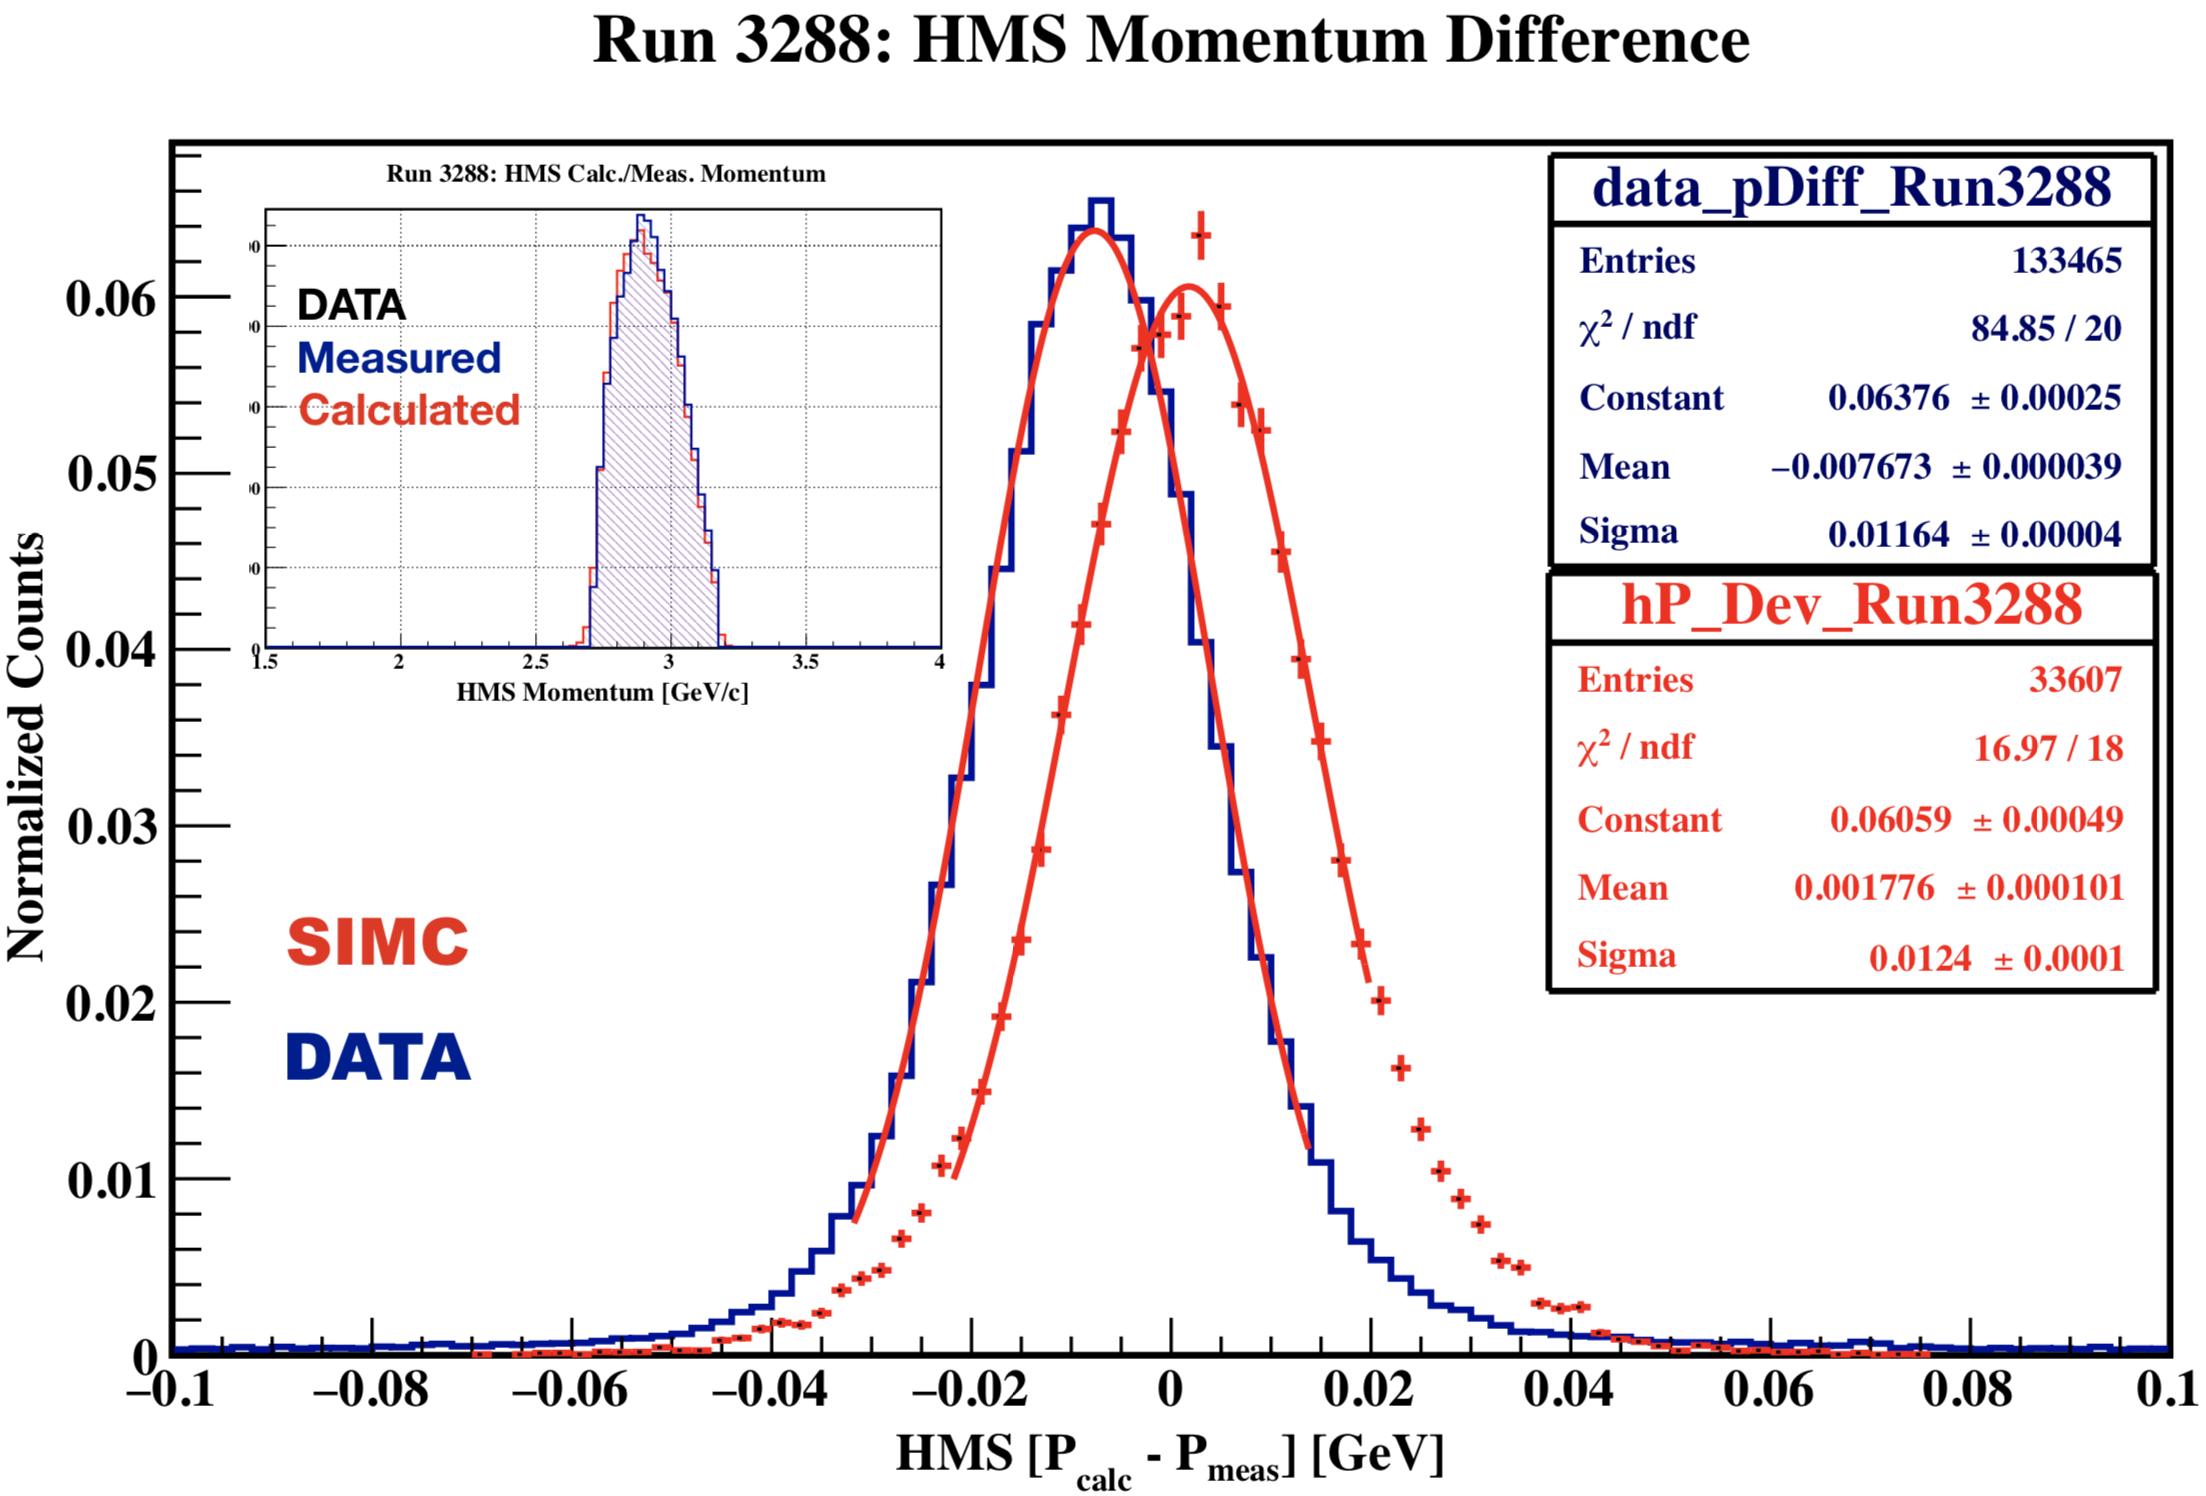
\includegraphics[scale=0.4]{plots/hms_Pdiff.png}
  \caption{Comparison of HMS momentum difference ($\Delta P$) between DATA and SIMC. The subplot shows the calculated and measured
  HMS momentum distribution for DATA.}
  \label{fig:hms_Pdiff}
\end{figure}\\
From the mean of the fit in Figure \ref{fig:hms_Pdiff}, $\Delta P_{DATA}$ is $\sim$8 MeV smaller than $\Delta P_{SIMC}$, or equivalently,
$P_{DATA}^{meas} > P_{DATA}^{calc}$. The data momentum correction factor can be determined from the following formula:
\begin{equation}
  f^{hms}_{corr} = 1 - \frac{\Delta P_{SIMC} - \Delta P_{DATA}}{P_{0}}
  \label{eq:4}
\end{equation}
and the corrected HMS momentum can be expressed as
\begin{equation}
  P^{HMS}_{corr} = P^{HMS}_{uncorr} \cdot f^{hms}_{corr}
  \label{eq:5}
\end{equation}
\begin{figure}[h!]
  \centering
  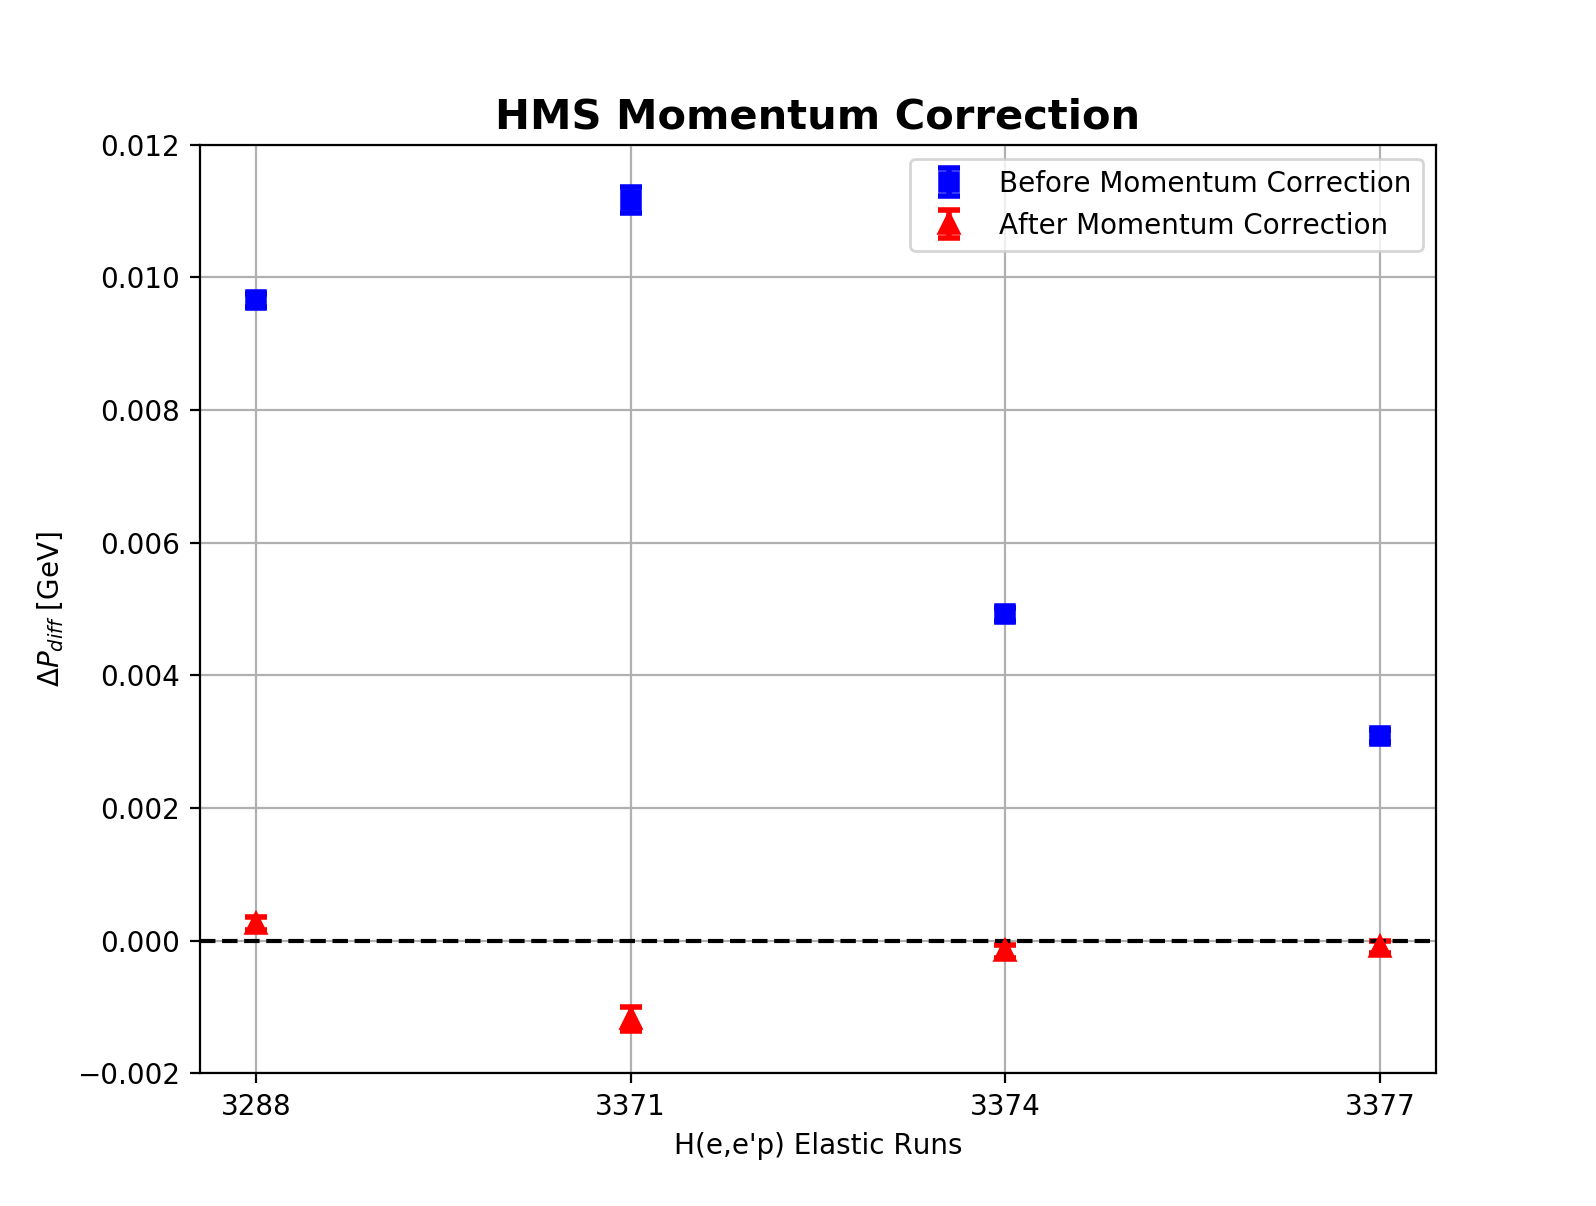
\includegraphics[scale=0.6]{plots/hms_Pcorr.png}
  \caption{HMS momentum difference, $\Delta P_{diff}=\Delta P_{SIMC} - \Delta P_{DATA}$, before and after applying the momentum correction to data.}
  \label{fig:hms_Pcorr}
\end{figure}\\
Figure \ref{fig:hms_Pcorr} shows the difference in the mean of the fit for DATA and SIMC before and after the HMS momentum
corrections. After correction, the difference between DATA and SIMC is within $\sim$1 MeV for the four elastic runs. It is important to note
that the corrections applied are after a second iteration, once the spectrometer offsets were determined. \\
\begin{figure}[h!]
  \centering
  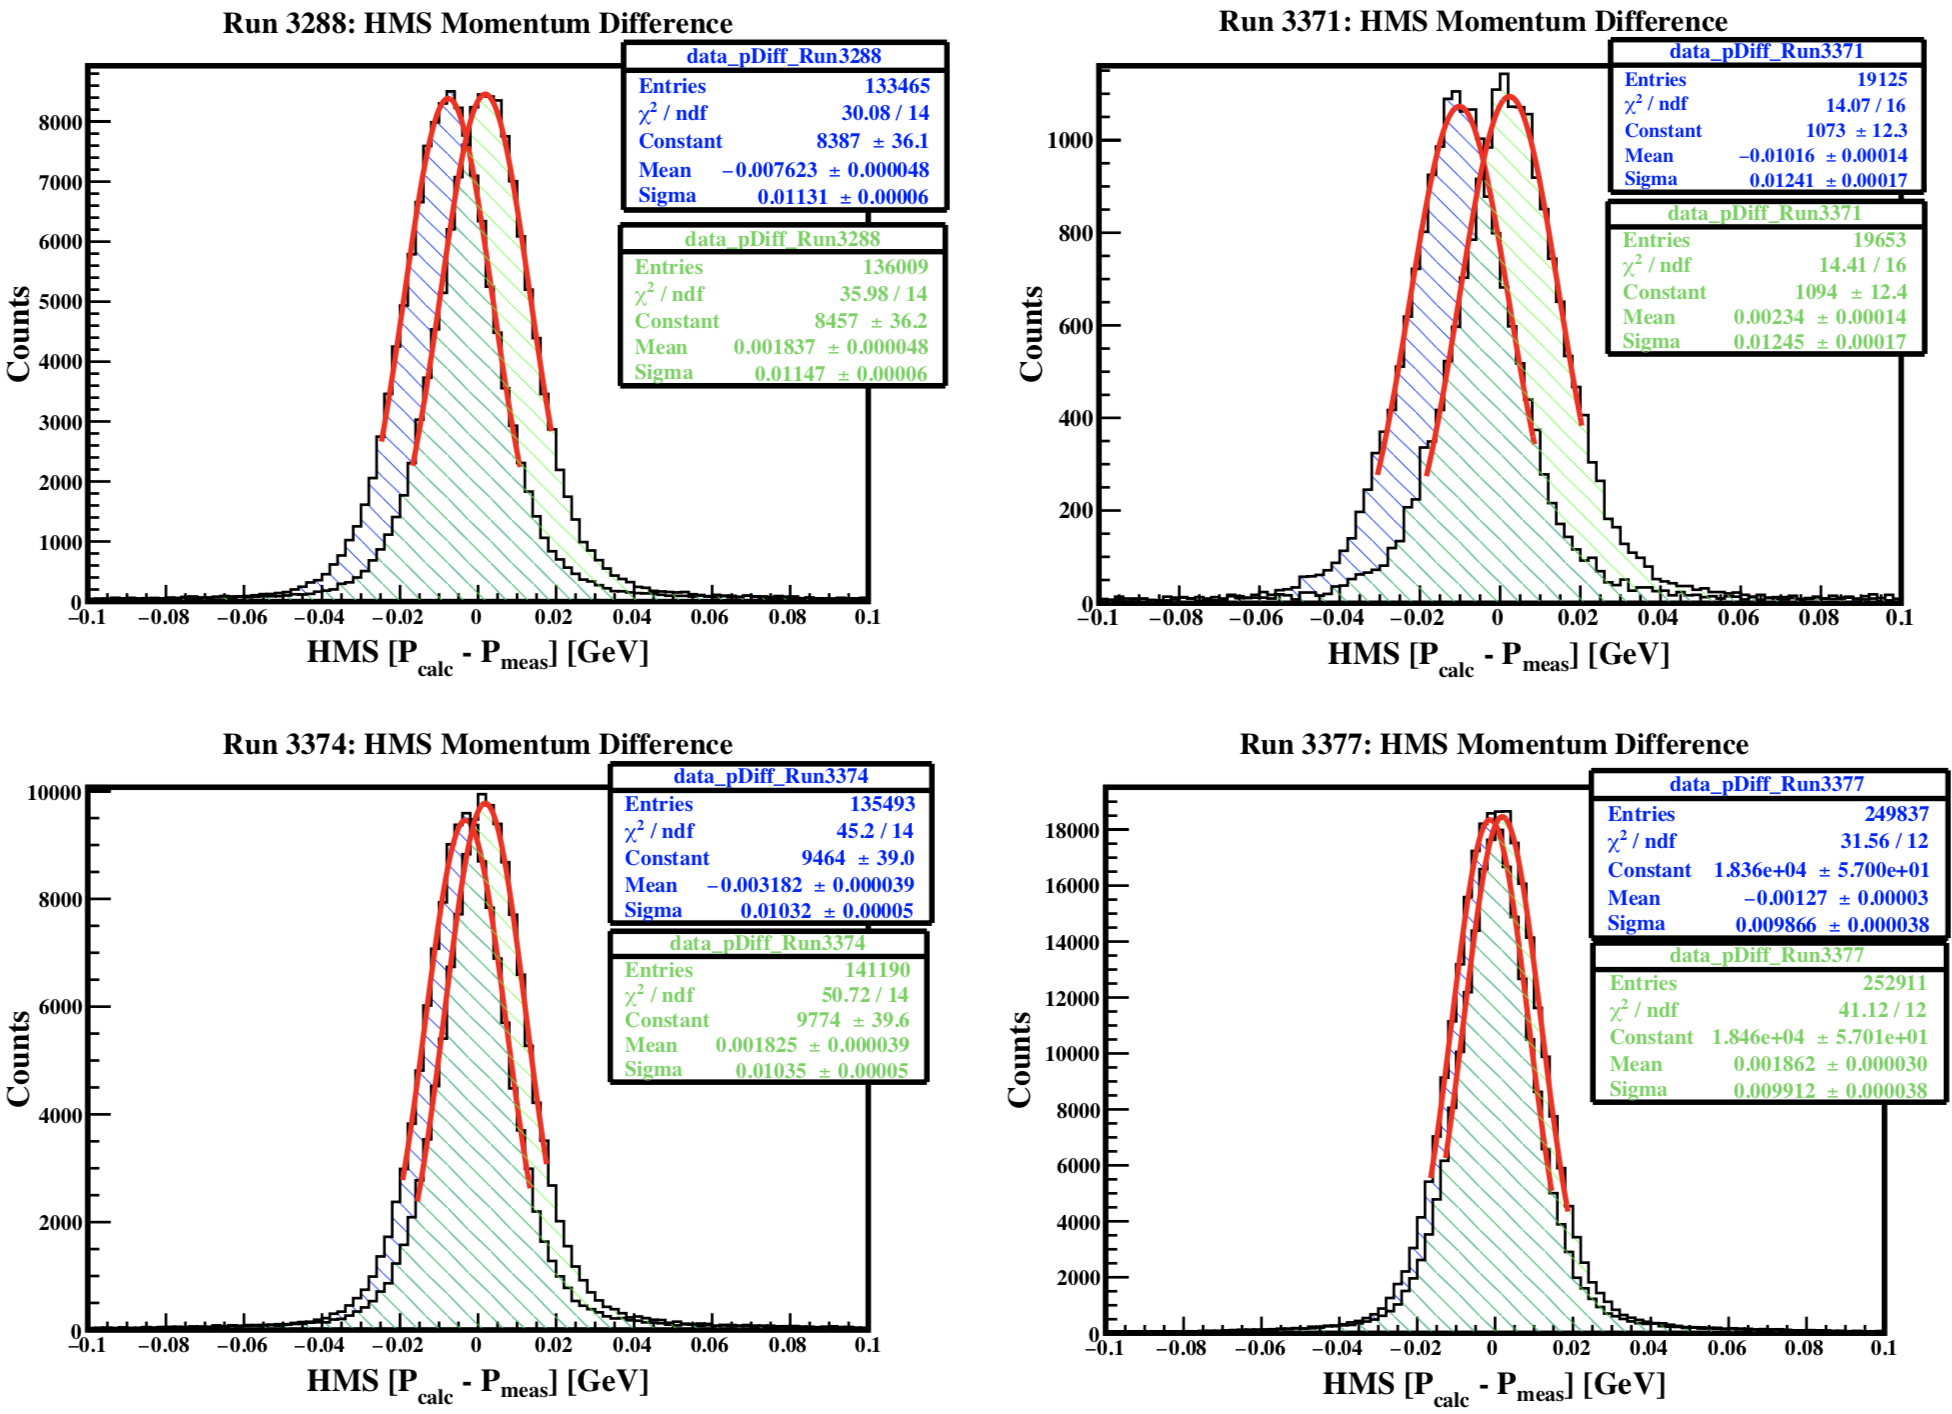
\includegraphics[scale=0.4]{plots/hms_dataPdiff_compare.png}
  \caption{HMS momentum difference for DATA, before (\textcolor{blue}{blue}) and after (\textcolor{green}{green}) applying the momentum correction ($2^{nd}$ iteration) to data.}
  \label{fig:hms_dataPdiff}
\end{figure}

\subsection{HMS $\delta$ Check }
To check the HMS Delta ($\delta$) reconstruction matrix, we plot the HMS fractional momentum difference defined as
\begin{equation}
\Delta P_{frac} = \frac{P_{calc} - P_{meas}}{P_{meas}}
\end{equation}
as a function of the HMS focal plane variables.  

\begin{figure}[h!]
  \centering
  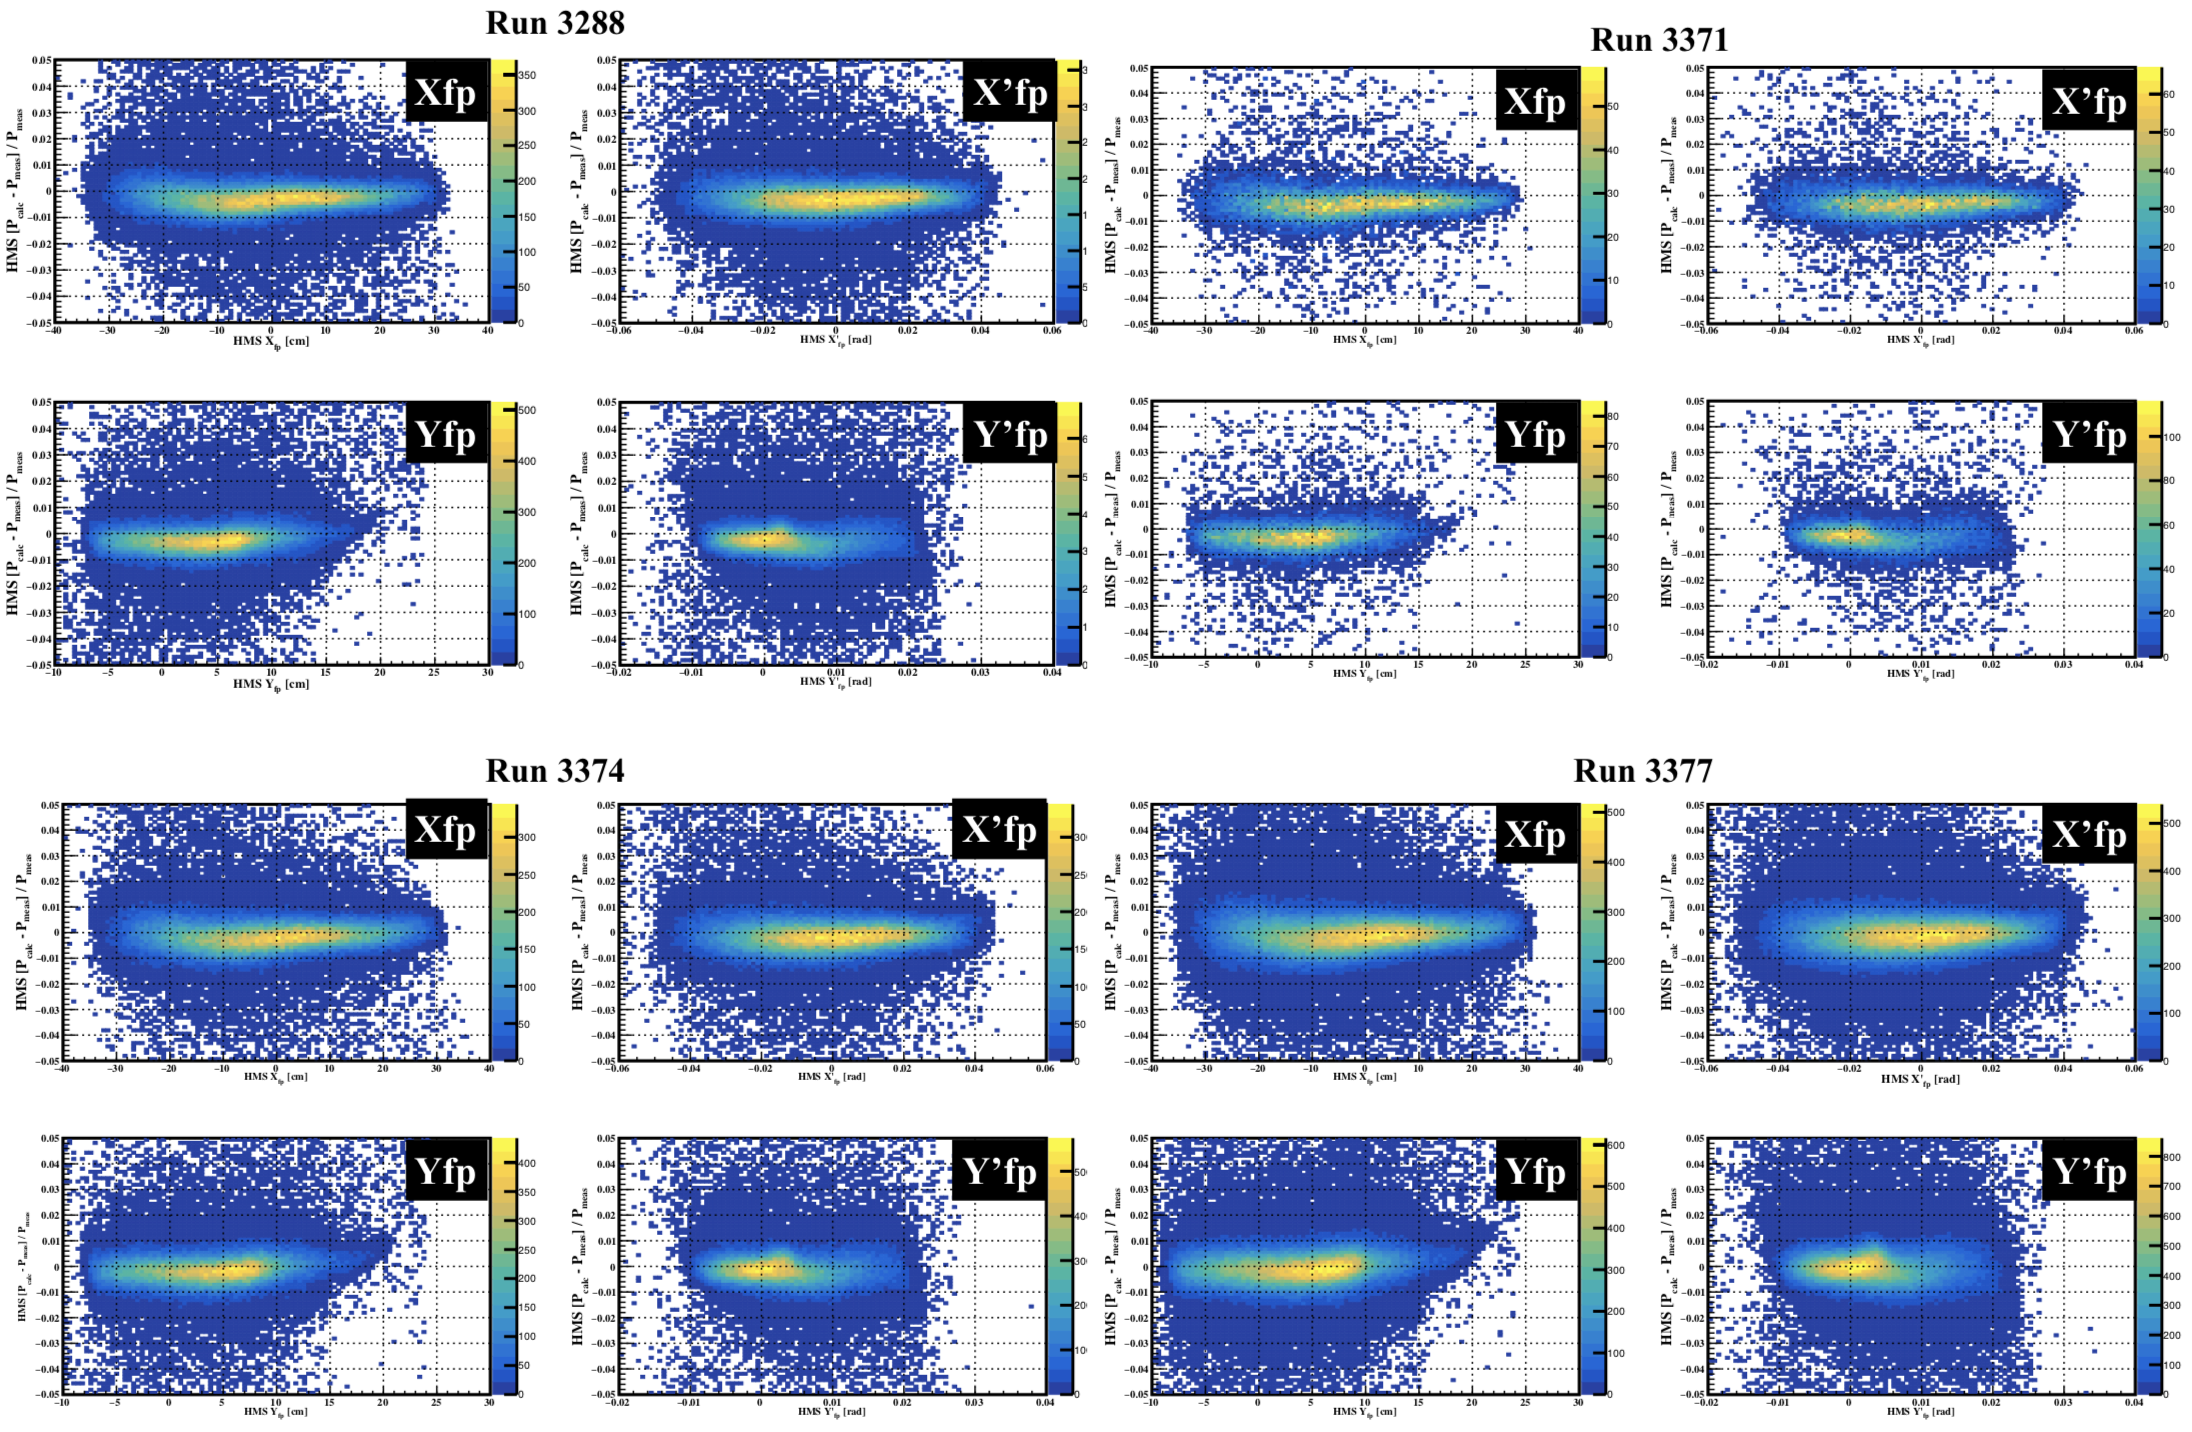
\includegraphics[scale=0.4]{plots/HMS_hPdiff_vs_FP.png}
  \caption{HMS fractional momentum difference vs. focal plane variables for the four H(e,e'p) Elastic runs.}
  \label{fig:hms_hPdiff_vs_FP}
\end{figure}
\noindent Figure \ref{fig:hms_hPdiff_vs_FP} shows the fractional HMS momentum is un-correlated across each of the
HMS focal plane variables, which demonstrates that the $\delta$-reconstruction matrix is already optimized
for the HMS. Now that we claim the HMS momentum and optics are well understood, we move on to the SHMS Checks.

\section{SHMS Optics Check}
Similarly to the HMS, the procedure to check the SHMS Optics involves determining the central momentum correction
and checking the SHMS $\delta$-reconstruction matrix is un-correlated with the SHMS focal plane variables. Additional
checks on the $Y_{tar}, Y'_{tar}$ and $X'_{tar}$ reconstruction variables may be needed as the SHMS Optics are still \textbf{NOT}
completely well understood.

\subsection{Central Momentum Correction}
To determine the SHMS central momentum correction, we start with the missing energy definition of H(e,e'p)
\begin{equation}
  E_{miss} = (E_{b} - E') + M_{p} - E_{p}
\end{equation}
where $E'$ and $E_{p}$ are the electron and proton final energies, respectively. Since it was assumed that
the beam energy is well known, and the HMS momentum has been corrected, any deviation from the expected missing
energy is attributed to the electron momentum in the SHMS. The expected location of the $E_{miss}$ ideally would
be at zero since H(e,e'p) is a completely determined system. However, due to the energy loss and radiative effects,
the peak has a small offset from zero ($\lesssim$10 MeV), which can only be simulated. The measured and simulated
$E_{miss}$ are then compared to determined if the SHMS central momentum needs to be corrected.
\begin{figure}[h!]
  \centering
  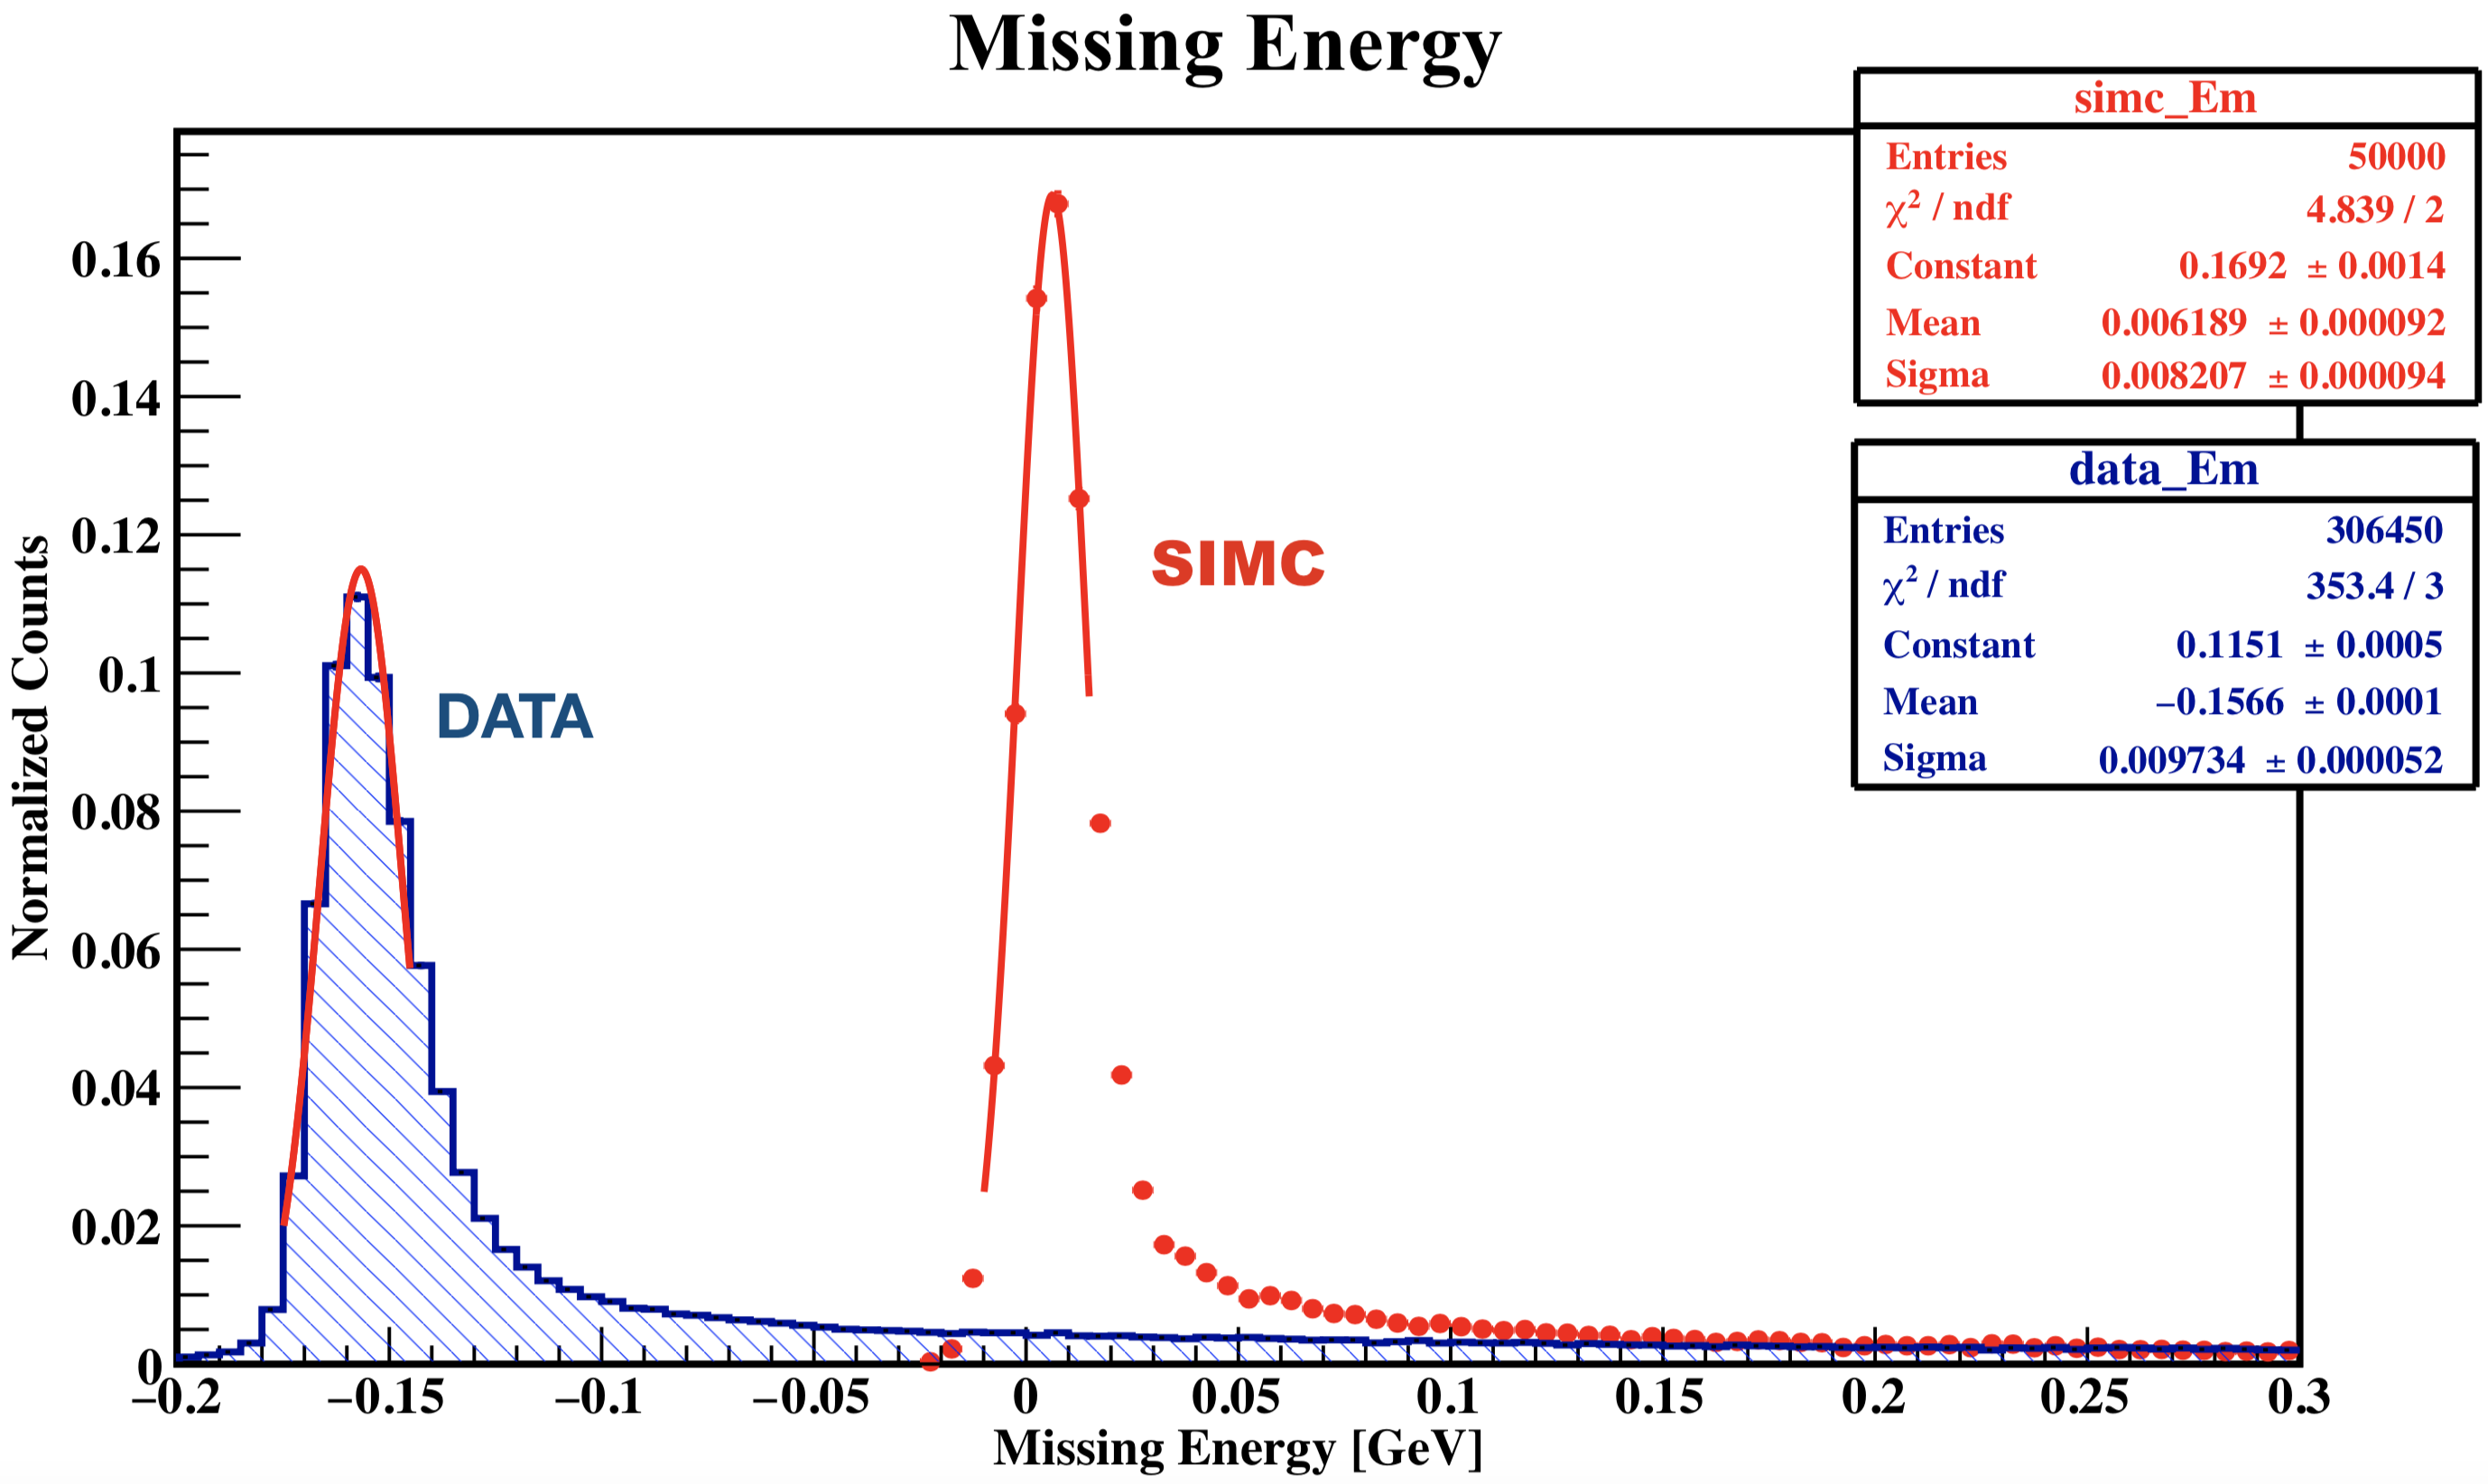
\includegraphics[scale=0.2]{plots/Emiss_3288_UnCorr.png}
  \caption{Missing Energy Spectrum for H(e,e'p) Elastic run 3288 before central momentum correction.}
  \label{fig:Emiss_UnCorr}
\end{figure} \\
The SHMS central momentum was kept fixed during the entire experiment, which would suggest that the missing
energy offset would be the same for the four elastic runs after the HMS momentum correction. This was found
\textbf{NOT} to be the case, however, due to the fact that the spectrometer offsets have not been determined
at this stage. Alternatively, it was decided to only focus on finding the central momentum correction
for run 3288, as it was the closest kinematic setting to the D(e,e'p) 80 MeV setting. This correction would then
be applied to the remaining elastic runs. \\
\indent Assuming any variation in missing energy between DATA and SIMC was due to the electron momentum, $E'$,
\begin{equation}
  \frac{\delta E_{miss}}{\delta E'} = -1 \rightarrow \delta E_{miss} = -\delta E' \\
\end{equation}
where $\delta E_{miss} = E^{SIMC}_{miss} - E^{DATA}_{miss}$ from the missing energy peak fit.
The electron momentum correction is then
\begin{align}
  E'_{corr} & =  E'_{uncorr} + \delta E' \nonumber \\
  & = E'_{uncorr}(1 - \frac{\delta E_{miss}}{E'_{uncorr}})
\end{align}
where the correction factor is
\begin{equation}
f^{shms}_{corr} = 1 - \frac{\delta E_{miss}}{E'_{uncorr}}
\end{equation}
After correcting the SHMS central momentum, the SHMS $\delta$-reconstruction also needs to be checked as a function
of the SHMS focal plane variables, as it may need to be optimized.
\subsection{SHMS $\delta$ Optimization}
To check the SHMS $\delta$-reconstruction matrix, similarly to the HMS, one needs to determined if there exists any
correlation of across the focal plane, as each of the reconstructed variables ($Y_{tar}$, $X'_{tar}$, $Y'_{tar}$, $\delta$) in general,
depends on a linear combination of the focal plane variables ($X_{fp}$, $X'_{fp}$, $Y_{fp}$, $Y'_{fp}$).
In general, the $\delta$ component can be expressed as
\begin{equation}
  \delta = \sum_{ijklm} D_{ijklm}x^{i}_{fp}x'^{j}_{fp}y^{k}_{fp}y'^{l}_{fp}x^{m}_{tar}
  \label{eq:11}
\end{equation}
where $i,j,k,l,m$ are the powers of the focal plane quantities and $D_{ijklm}$ are the matrix
coefficients for a particular combination of powers. \\
\indent To optimize the $\delta$-component, we define calculated $\delta$ as
\begin{equation}
  \delta_{calc} = \frac{P_{calc} - P_{0}}{P_{0}} 
\end{equation}
where the calculated electron momentum is determined from momentum conservation to be
\begin{equation}
  P_{calc} = E_{b} + M_{p} - E_{p}, \text{ where } E_{p} = \sqrt{P_{meas}^{2} + M_{p}^{2} } \text{   and   } E_{calc} \sim P_{calc}
\end{equation}
The measured proton momentum, $P_{meas}$, is the corrected HMS momentum determined in the previous
section.
Taking the difference between the calculated and measured momentum,
\begin{equation}
  \chi^{2} \equiv (\delta_{calc} (E_{b}, P_{meas}) - \delta_{meas} (x_{fp}, x'_{fp}, y_{fp}, y'_{fp}))^{2}
  \label{eq:14}
\end{equation}
From Equation \ref{eq:14}, the SHMS $\delta$-optimization is now a $\chi^{2}$-minimization problem, where the goal is
to find a set of matrix coefficients,  $D_{ijklm}$, that minimizes the difference between the calculated and measured
$\delta$. For more further details, see Section 6 of \cite{HMS_notes} \\
\indent The $\chi^{2}$-minimization was done on all four elastics simultaneously, as each of them covered
a different (also overlapping) region of the SHMS $\delta$-reconstructed variable, such that the D(e,e'p)n data would be
inside the coverage. Additionally, \text{ONLY} the $(x_{fp}, x'_{fp})$ focal plane terms were used in the fit since
with elastic events there is a kinematic correlation between the momentum and scattering angle which translates into a correlation
between $x_{fp}$ and $(y'_{fp}, y_{fp})$. So if one fits $(y'_{fp}, y_{fp})$ then one can be fitting this kinematic
correlation and not an optics correlation \cite{priv_comm}.
\begin{figure}[h!]
  \centering
  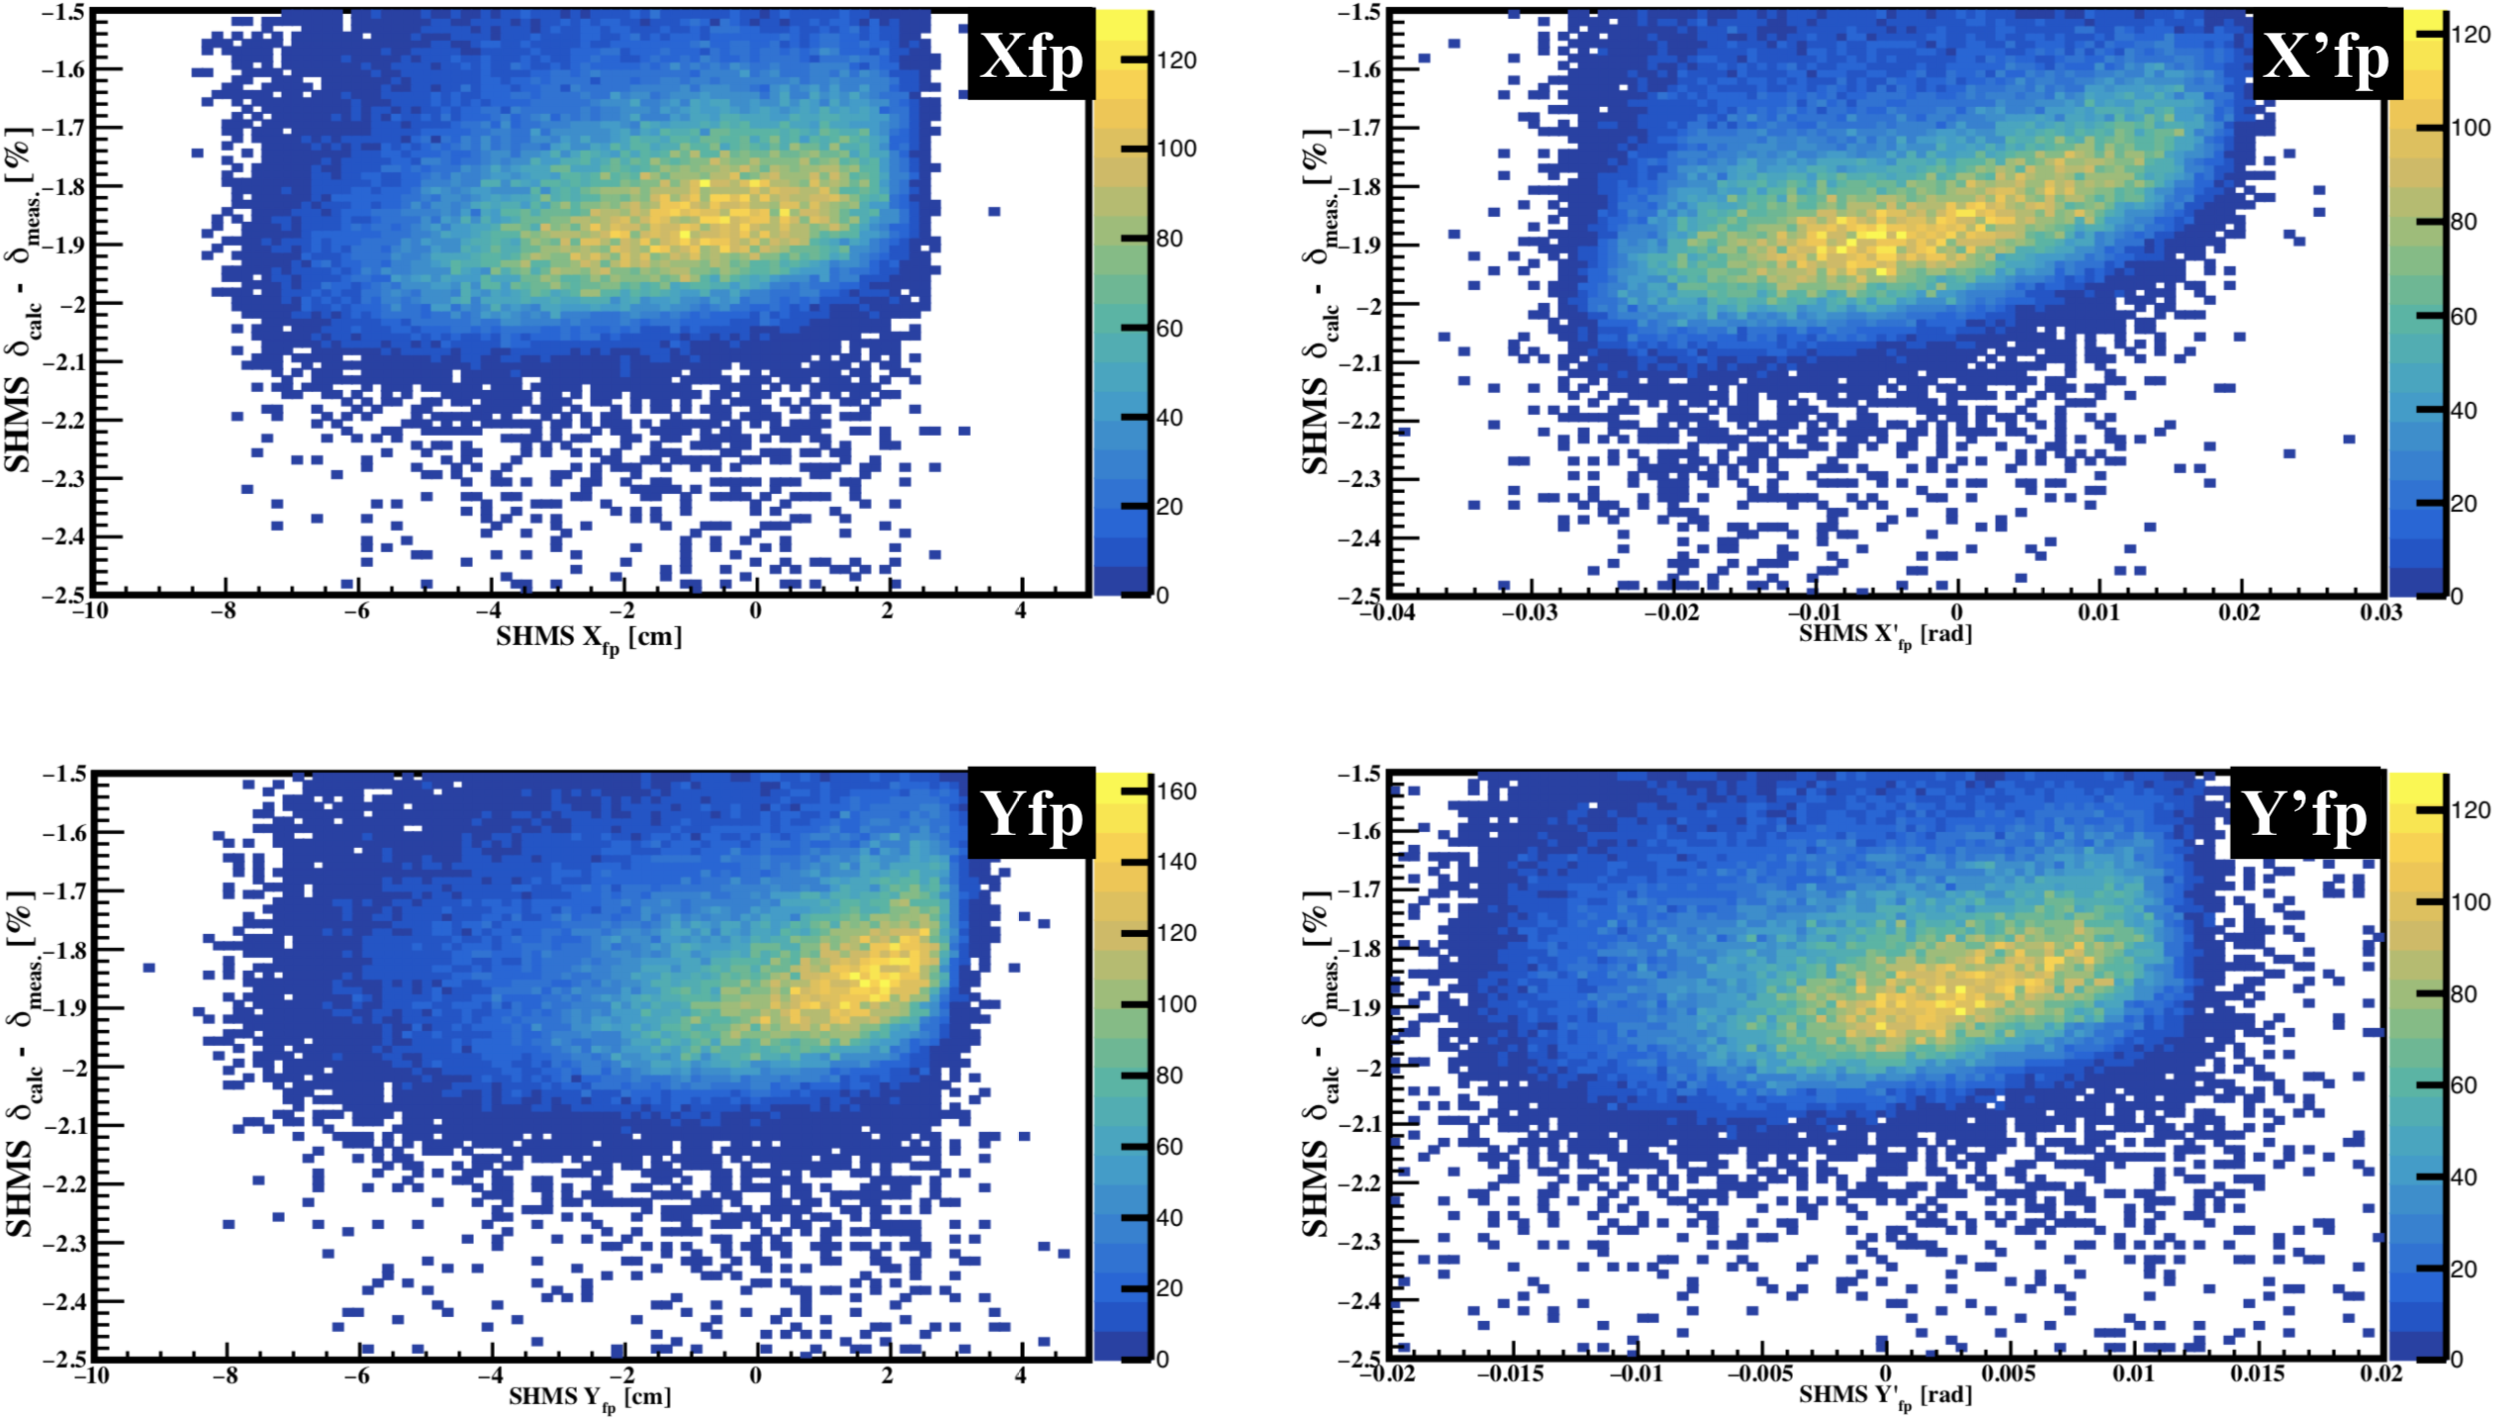
\includegraphics[scale=0.34]{plots/SHMS_DeltaDiff_BeforeOptim3288.png}
  \caption{SHMS $(\delta_{calc}-\delta_{meas})$ vs. focal plane variables for H(e,e'p) Elastic run 3288 before $\delta$-optimization.}
  \label{fig:shmsDelta_beforeOptim}
\end{figure}
\newpage
\indent The $\delta$ terms that were used in the fit can be expanded from Eq. \ref{eq:11},
\begin{equation}
  \delta_{meas} = D_{10000}\cdot x_{fp} + D_{01000}\cdot x'_{fp} + D_{11000}\cdot x_{fp}\cdot x'_{fp} + D_{20000}\cdot x^{2}_{fp} + D_{02000}\cdot x'^{2}_{fp}
\end{equation}
The coefficents were optimized for the first and second order $(x_{fp}, x'_{fp})$ terms as well as for the cross terms, as the correlations
observed were not completely linear, as shown in the Figure \ref{fig:shmsDelta_beforeOptim}. After fitting the correlations and determining
the optimum coefficients, these were updated in the SHMS optics parameter file, and the data was replayed again.
\begin{figure}[h!]
  \centering
  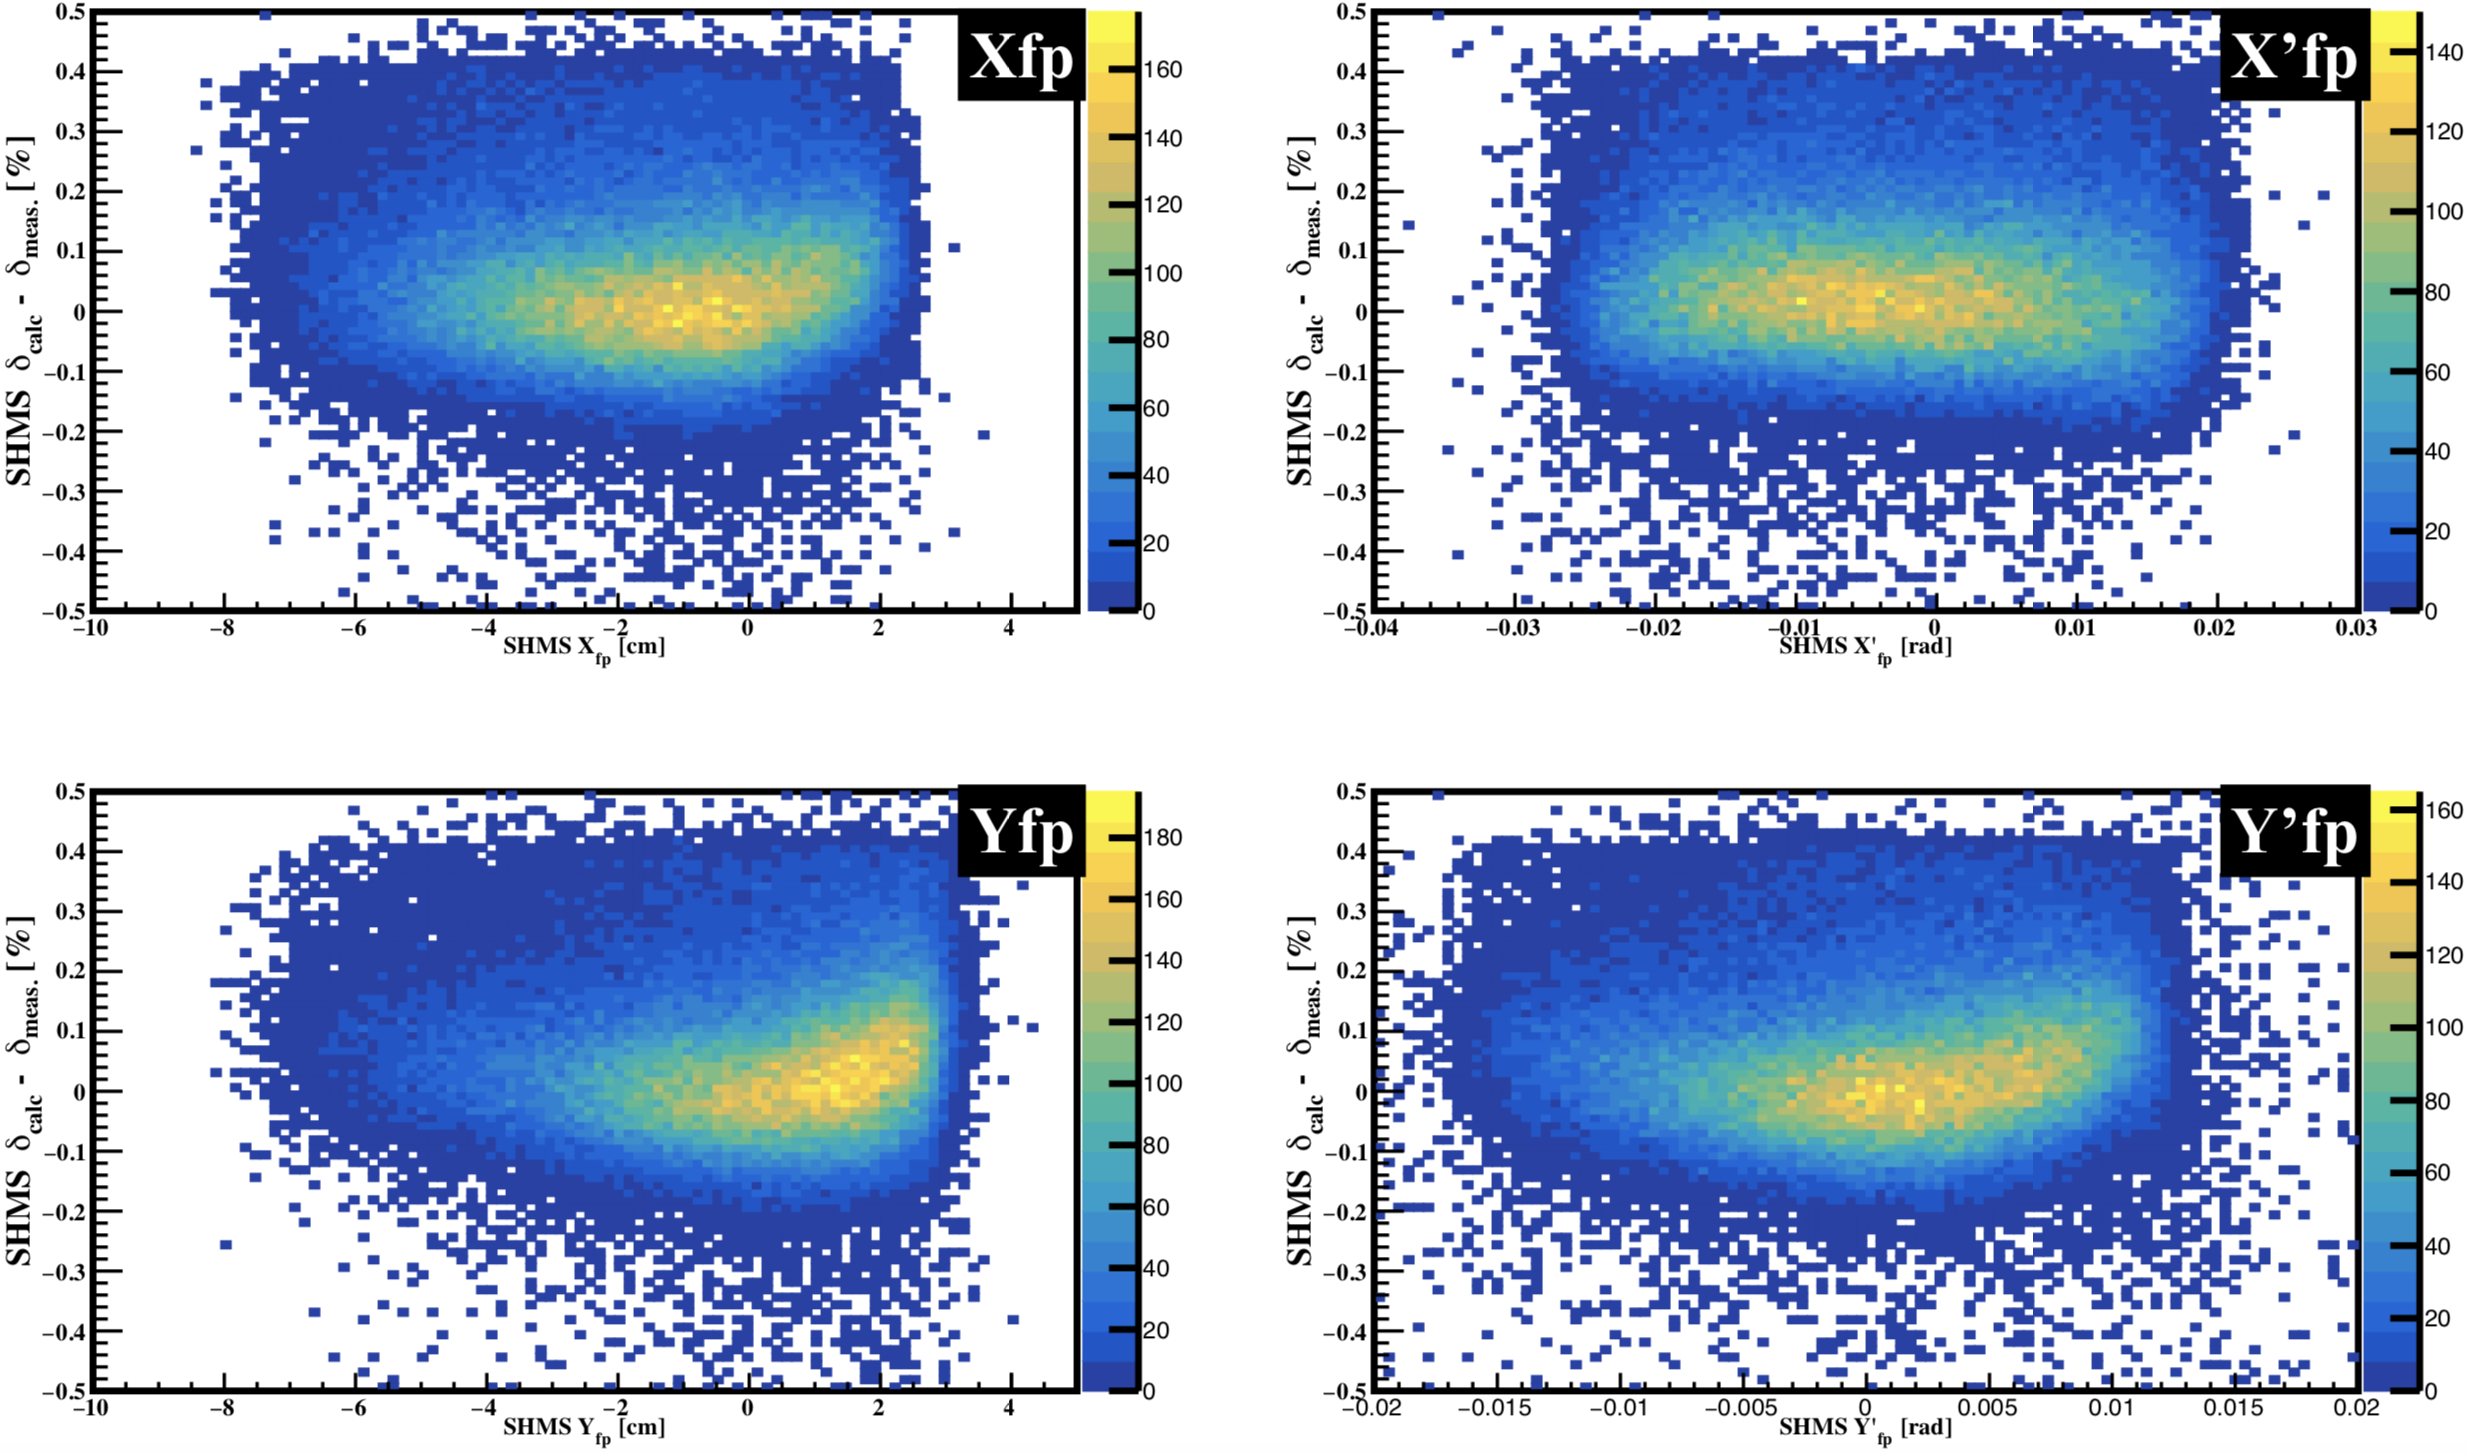
\includegraphics[scale=0.34]{plots/SHMS_DeltaDiff_AfterOptim3288.png}
  \caption{SHMS $(\delta_{calc}-\delta_{meas})$ vs. focal plane variables for H(e,e'p) Elastic run 3288 after $\delta$-optimization.}
  \label{fig:shmsDelta_afterOptim}
\end{figure}\\
From Figure \ref{fig:shmsDelta_afterOptim}, there is a noticeable improvement in the $(x_{fp}, x'_{fp})$, as the correlations have
been corrected, whereas in the $(y_{fp}, y'_{fp})$, the effect is less noticeable as these were not involved in the fit. 
\begin{figure}[h!]
  \centering
  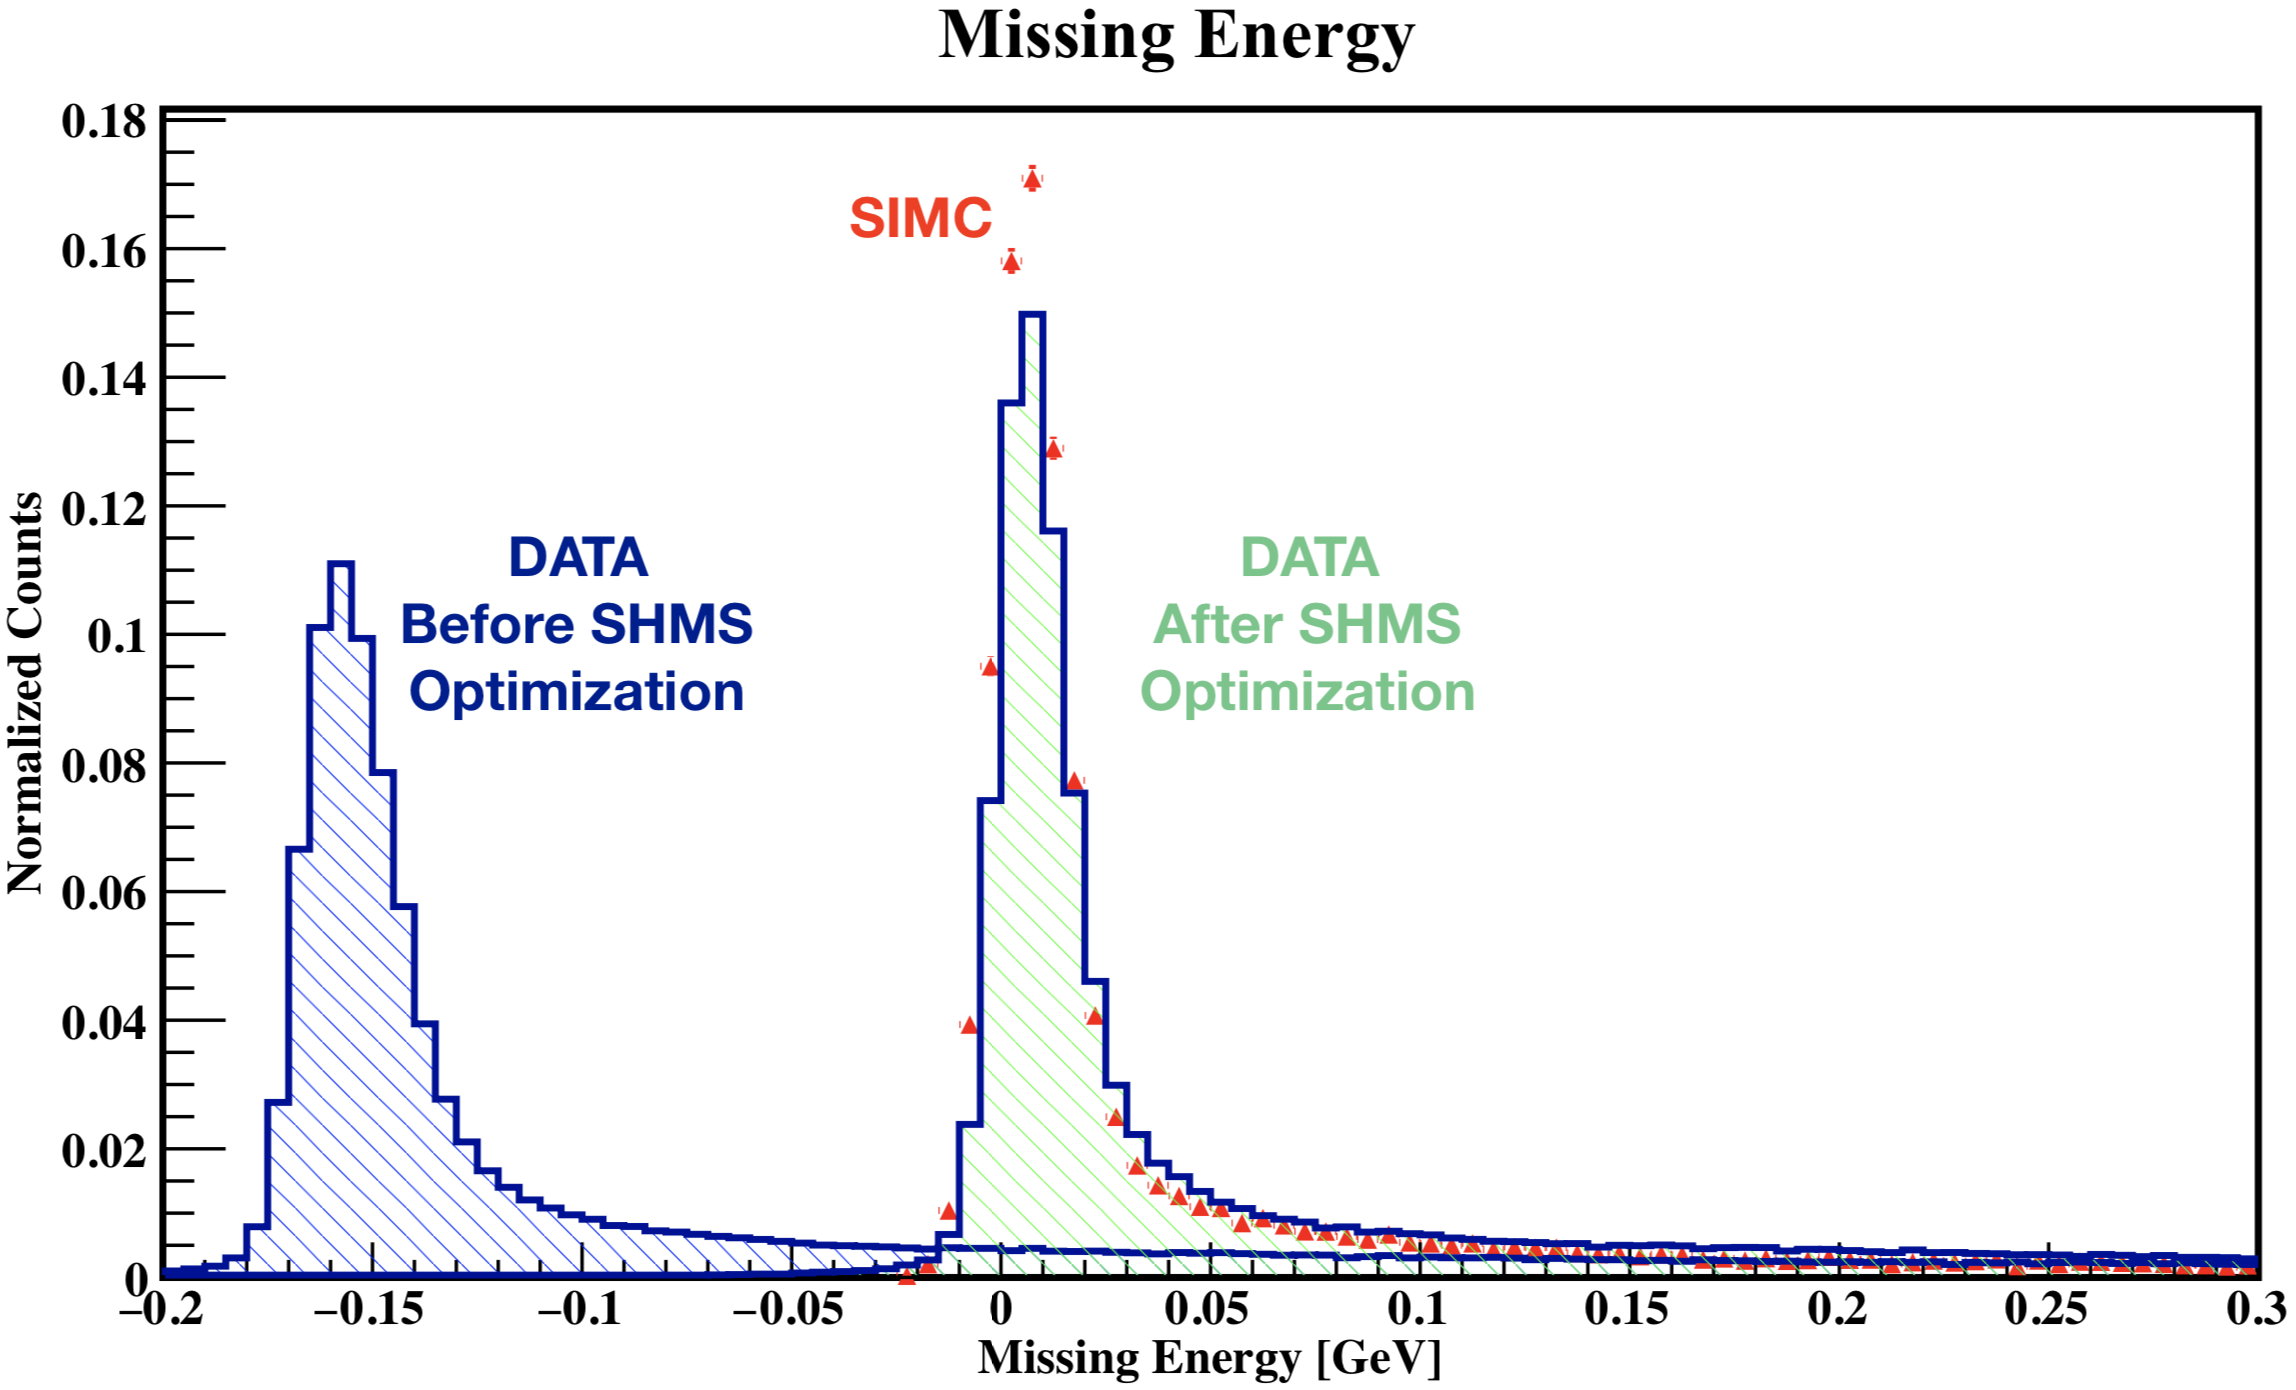
\includegraphics[scale=0.3]{plots/Emiss_3288_FullOptim.png}
  \caption{Missing Energy Spectrum for H(e,e'p) Elastic run 3288 after central momentum correction and $\delta$-optimization.}
  \label{fig:shmsEm_afterOptim}
\end{figure}
\newpage
\indent From Figure \ref{fig:shmsEm_afterOptim}, after the SHMS central momentum correction and optimization, there
is a clear improvement in the missing energy spectrum. The improvents observed are
\begin{itemize}
\item Alignment of DATA Missing Energy to SIMC from the central momentum correction
\item Narrower width in DATA Missing Energy from $\delta$-optimization of the matrix coefficients.
\end{itemize}
The first bullet point is easy to understand, as the alignment is simply due to a change in the SHMS central momentum.
The second bullet point can be understood from the fact that since the SHMS $\delta_{meas}$ matrix coefficients
\footnote{The SHMS $\delta$ matrix coefficients are directly associated with the SHMS measured momentum on an event-by-event
  basis, so if these coefficients are optimized, the measured SHMS momentum is optimized, which directly affects where the
  Missing Energy event will be reconstructed.}
have been optimized, an event in the missing energy spectrum that would otherwise be reconstructed far away from the
main peak, is now reconstructed underneath the main peak resulting in an improvement in the resolution as well as in
the recovered events. 
\subsection{SHMS $(Y_{tar}, Y'_{tar}, X'_{tar})$ Optimization}
During the E12-10-003 experiment, an Optics run with the Centered Sieve was taken after the optics in SHMS Q3 were fixed. This data was used to
optimize the $(Y_{tar}, Y'_{tar}, X'_{tar})$ components of the reconstruction matrix. The target consists of three Carbon foils positioned at
(-10, 0, 10) cm to mimic the target Hall C target edges and center. The reconstructed the events back to each of the foils serve to check the optics.
The optimization code used is located at github repository \cite{shmsOpt_git_repo}. \\
\indent To check the optics, the SHMS $\delta$ vs. $Y_{tar}$ was plotted to verify how well is the $Y_{tar}$ reconstructed across $\delta$ for each of the
three foils. Below are the plots showing before and after the optimization.
\begin{figure}[h!]
  \centering
  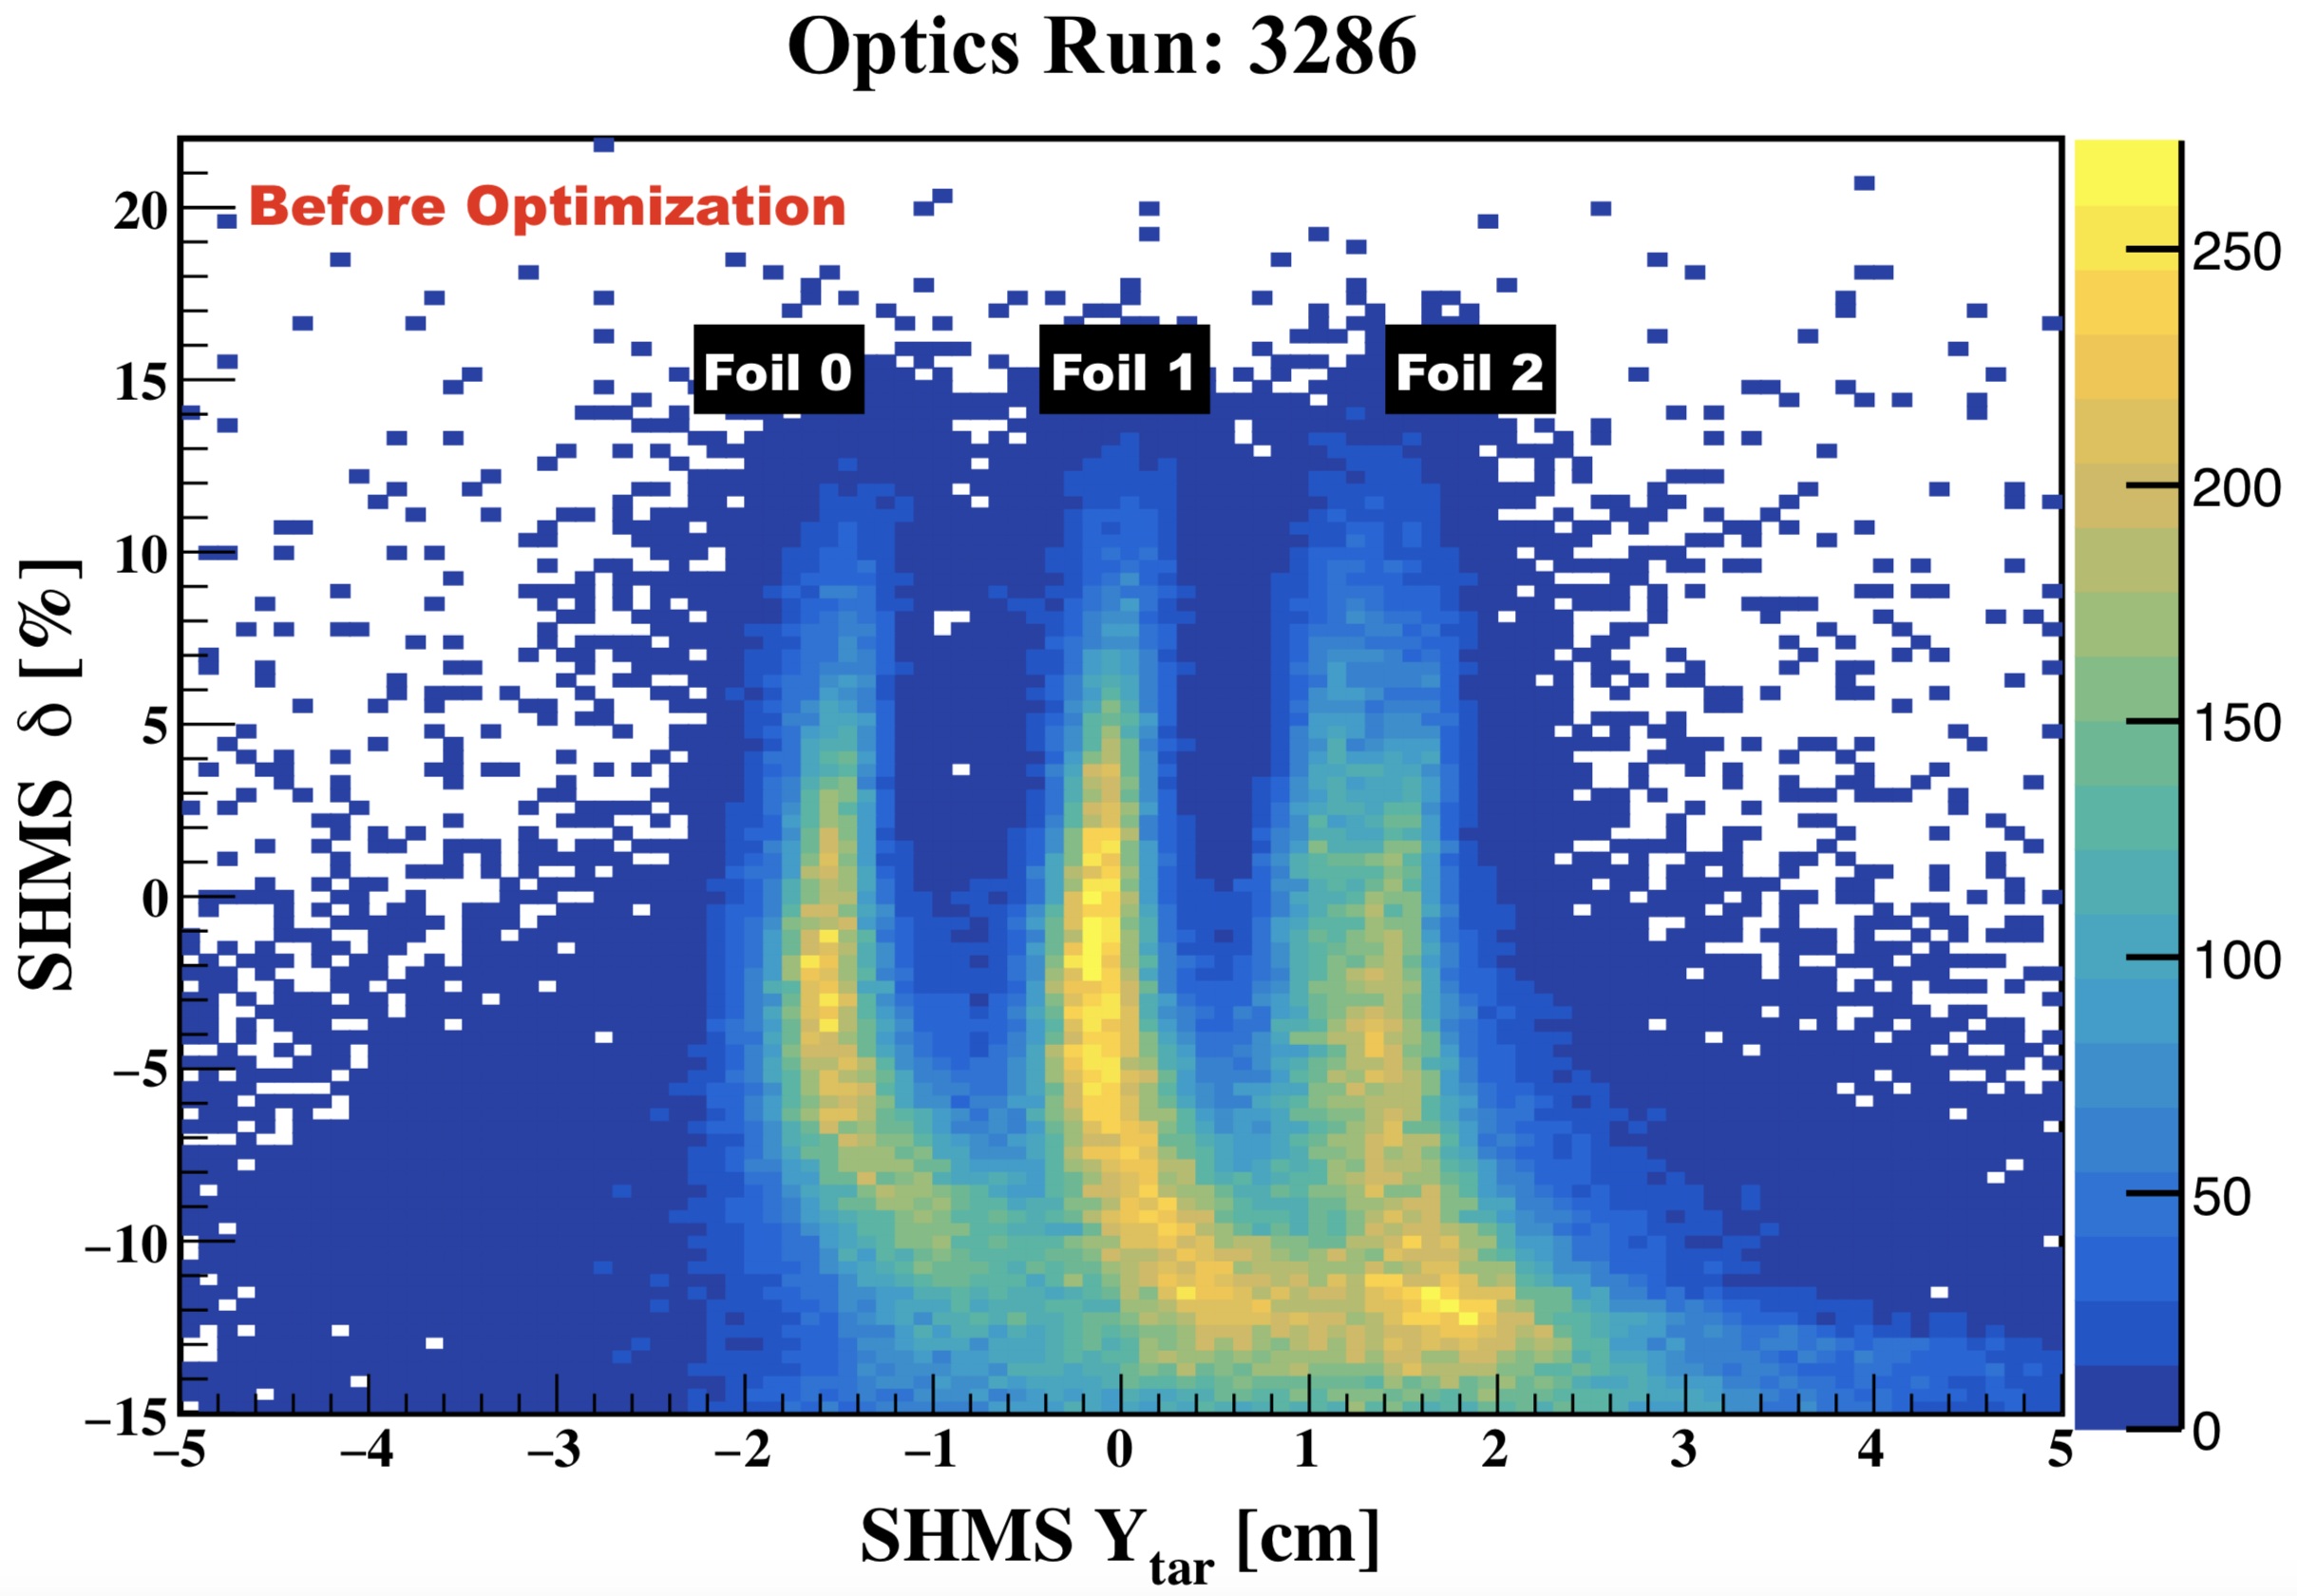
\includegraphics[scale=0.4]{plots/SHMS_delta_vs_ytar_3286_beforeOptim.png}
  \caption{SHMS $\delta$ vs. $Y_{tar}$ for Carbon Sieve run 3286 before $Y_{tar}$-optimization.}
  \label{fig:shmsYtar_beforeOptim}
\end{figure}
\newpage
\begin{figure}[h!]
  \centering
  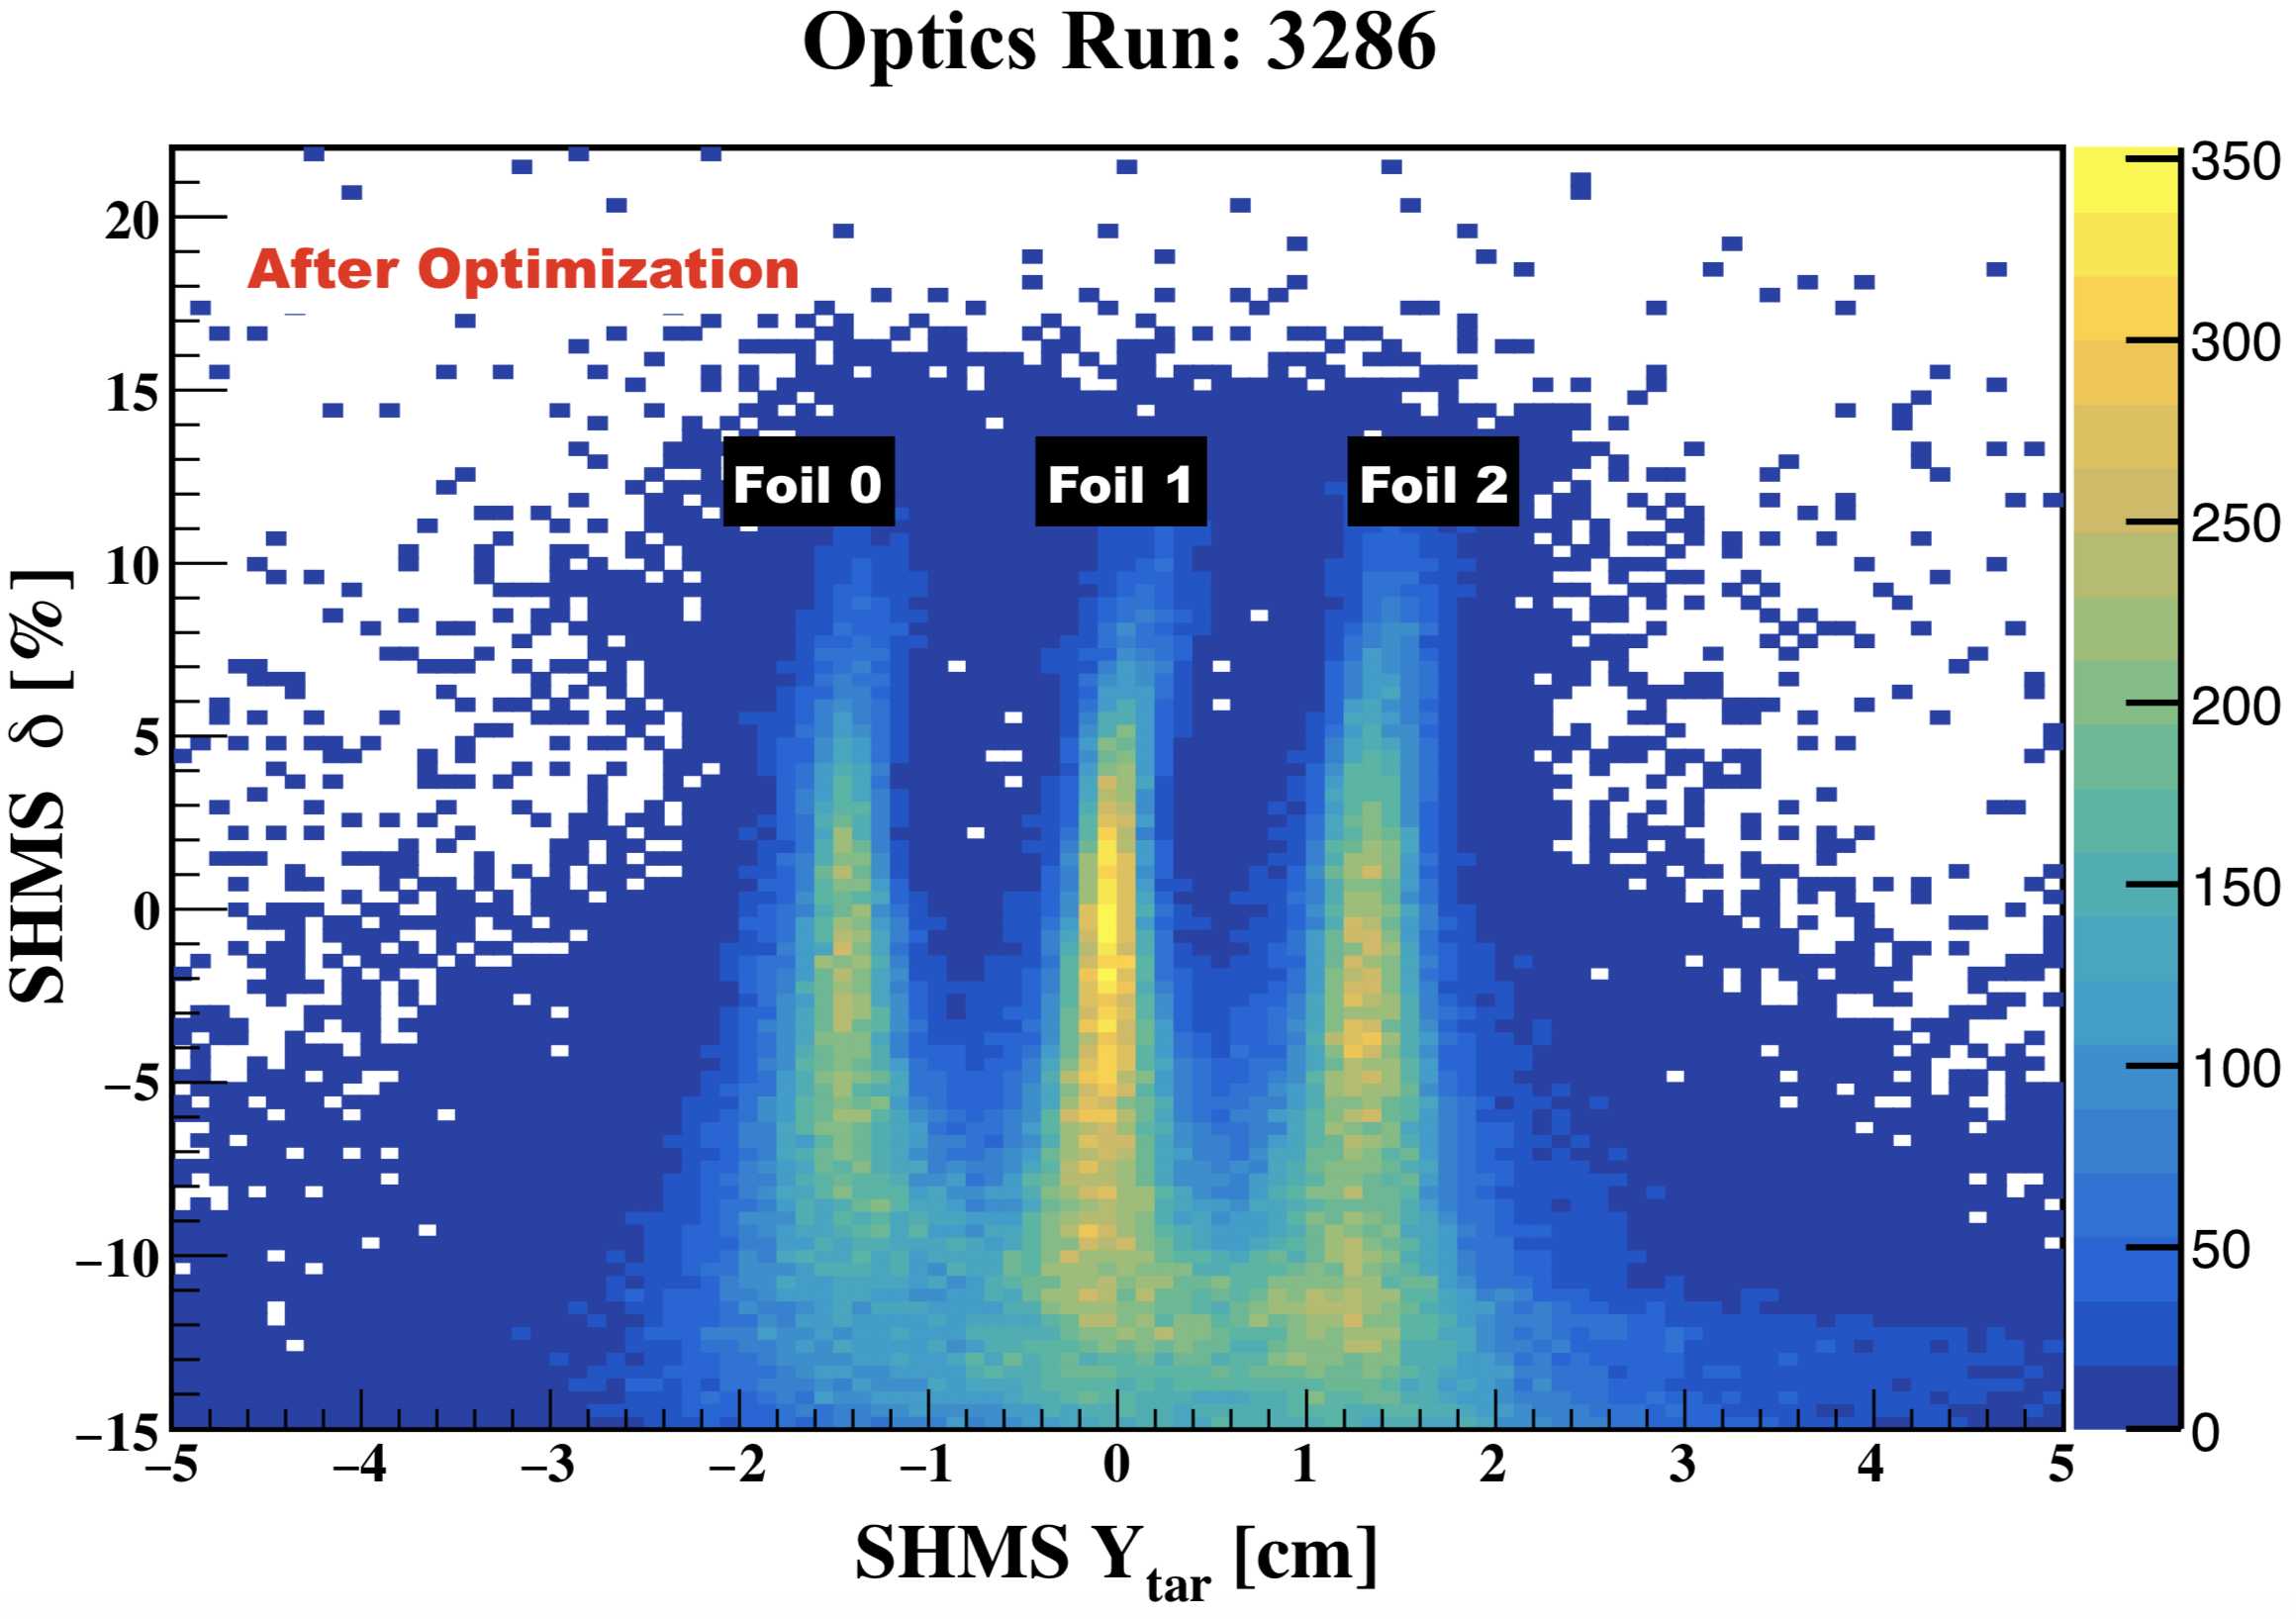
\includegraphics[scale=0.4]{plots/SHMS_delta_vs_ytar_3286_afterOptim.png}
  \caption{SHMS $\delta$ vs. $Y_{tar}$ for Carbon Sieve run 3286 after $Y_{tar}$-optimization.}
  \label{fig:shmsYtar_afterOptim}
\end{figure}
After the optimization, it is clear from Figure \ref{fig:shmsYtar_afterOptim} that there is almost no
correlation as compared to before optimization. The variables optimized, $(Y_{tar}, Y'_{tar}, X'_{tar})$ are
related to the in-plane and out-of-plane angles relative to the spectrometer central ray, so removing the correlation
in $Y_{tar}$ affects the the SHMS electron scattering angle. This in turn affects the location of the invariant mass peak as it depends
on the electron angle.
\section{Spectrometer Offstes} \label{sec:spec_off_sec}
\noindent The optics optimization was originally done assuming there were no spectrometer offsets. This is not true,
however, as there were still some small mis-alignments observed in the missing energy spectrum. An extensive study
of the spectrometer offsets in Hall C has not been done yet. For now, we have made a rough estimate on these
offsets based on observations in H(e,e'p) elastic run 3288, as it is closest in kinematic to the Deuteron 80 MeV setting.
\subsection{Central Angle Offsets}
\noindent The central angle offsets refer to the central ray spectrometer offsets in two cases:
\begin{itemize}
\item \textit{In-plane central angle offset} \texttt{[h(p)thetacentral\_offset]\footnote{The spectrometer offsets parameters can be found on \texttt{hallc\_replay/PARAM/(S)HMS/GEN/(s)hmsflags.param} \\ In general, it is not possible to know from which spectrometer is the offset originating, so the HMS was chosen in this case.}}
\item \textit{Out-of-plane central angle offset} \texttt{[h(p)\_oopcentral\_offset]}
\end{itemize}
The \textit{in-plane} is parallel to the Hall C floor, whereas the \textit{out-of-plane} is perpendicular to the Hall C floor.
The central angle offsets can be determined from the missing momentum components for H(e,e'p) elastics, as these should ideally be centered around
zero. In Hall Coordinate System (HCS), the in-plane central angle offset can be determined by taking the fractional dfference between
the measured (DATA) and expected (SIMC) X missing momentum component as follows:
\begin{equation}
  \delta \theta = \frac{P_{mx}^{SIMC} - P_{mx}^{DATA}}{P_{0}}
\end{equation}
The out-of-plane central angle offset can be determined by taking the fractional dfference between
the measured (DATA) and expected (SIMC) Y missing momentum component as follows:
\begin{equation}
  \delta \phi = \frac{P_{my}^{SIMC} - P_{my}^{DATA}}{P_{0}}
\end{equation}
\begin{figure}[h!]
  \centering
  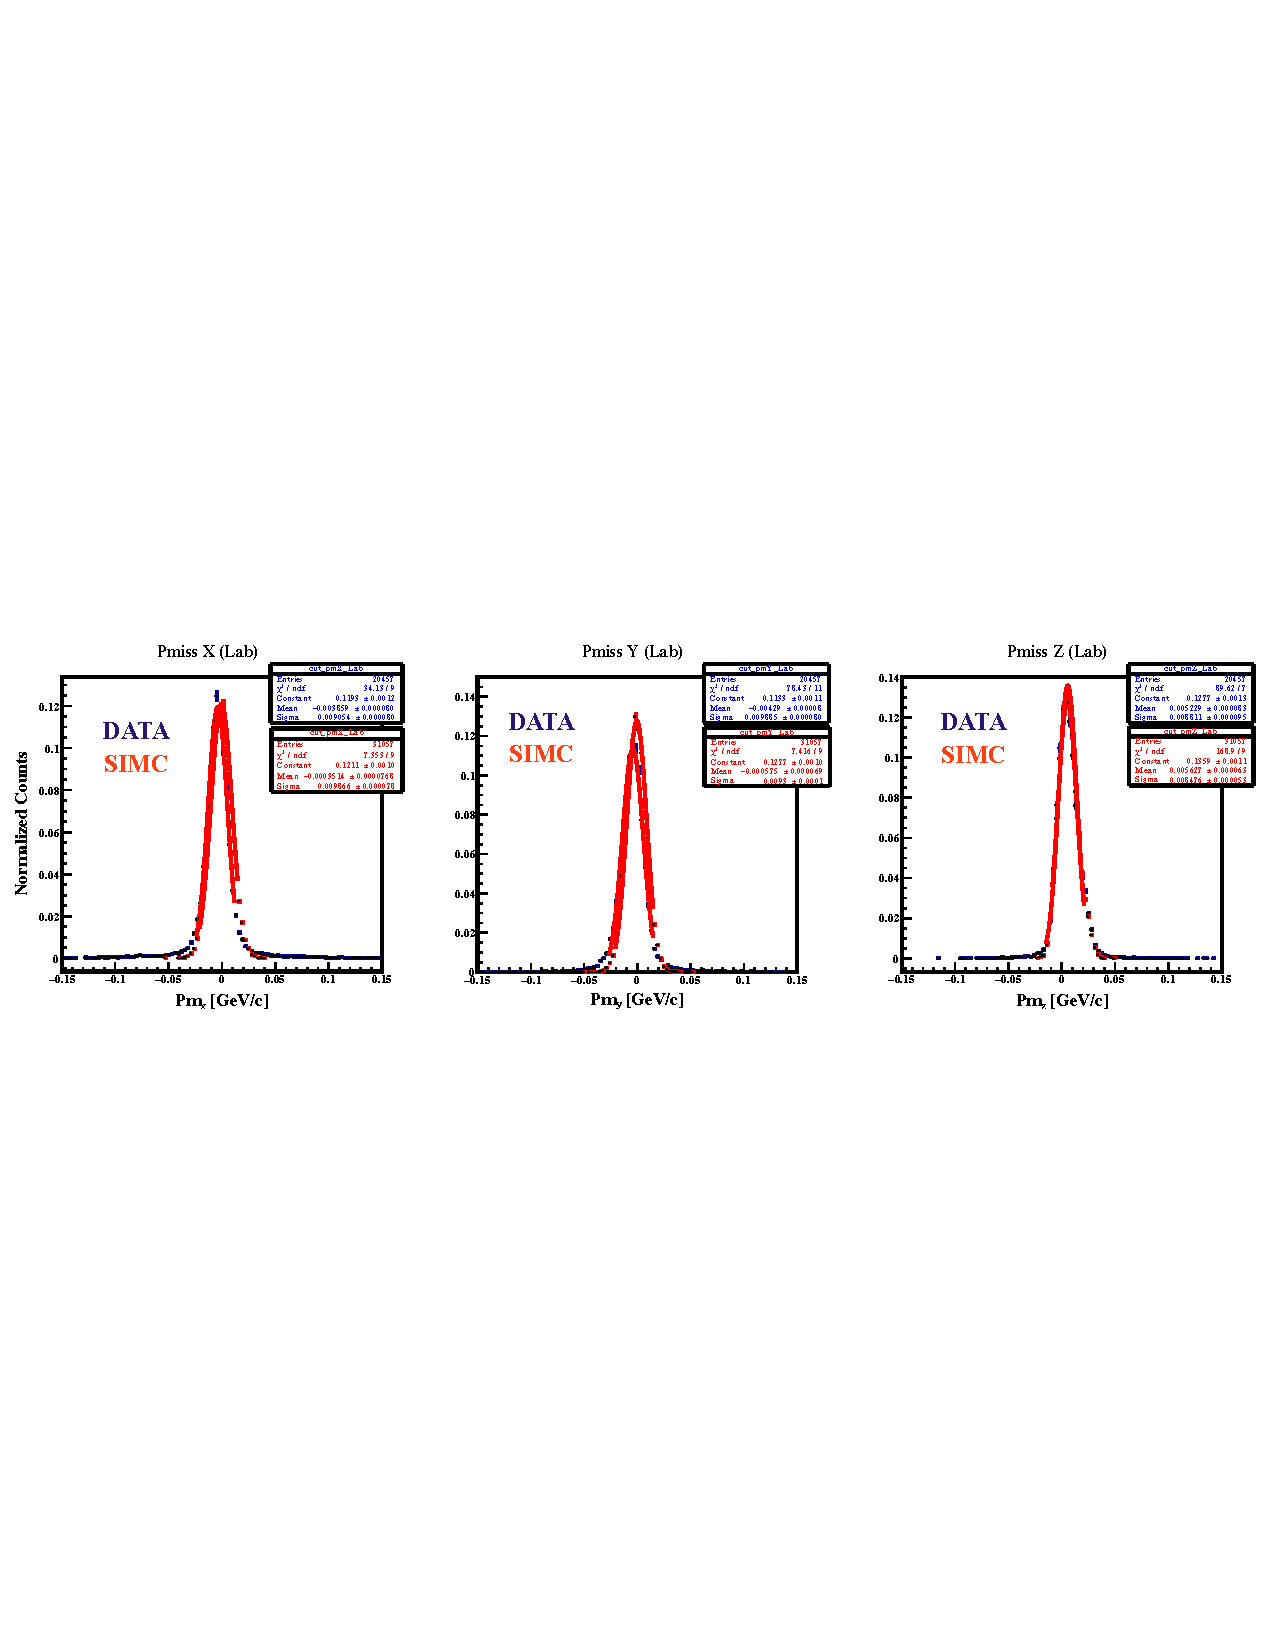
\includegraphics[scale=0.9]{plots/ORIGINAL_Pm_NOSpecOffsets.pdf}
  \caption{Missing Momentum components with NO spectrometer offsets applied.}
  \label{fig:PmComp_noOffsets}
\end{figure}
\begin{figure}[h!]
  \centering
  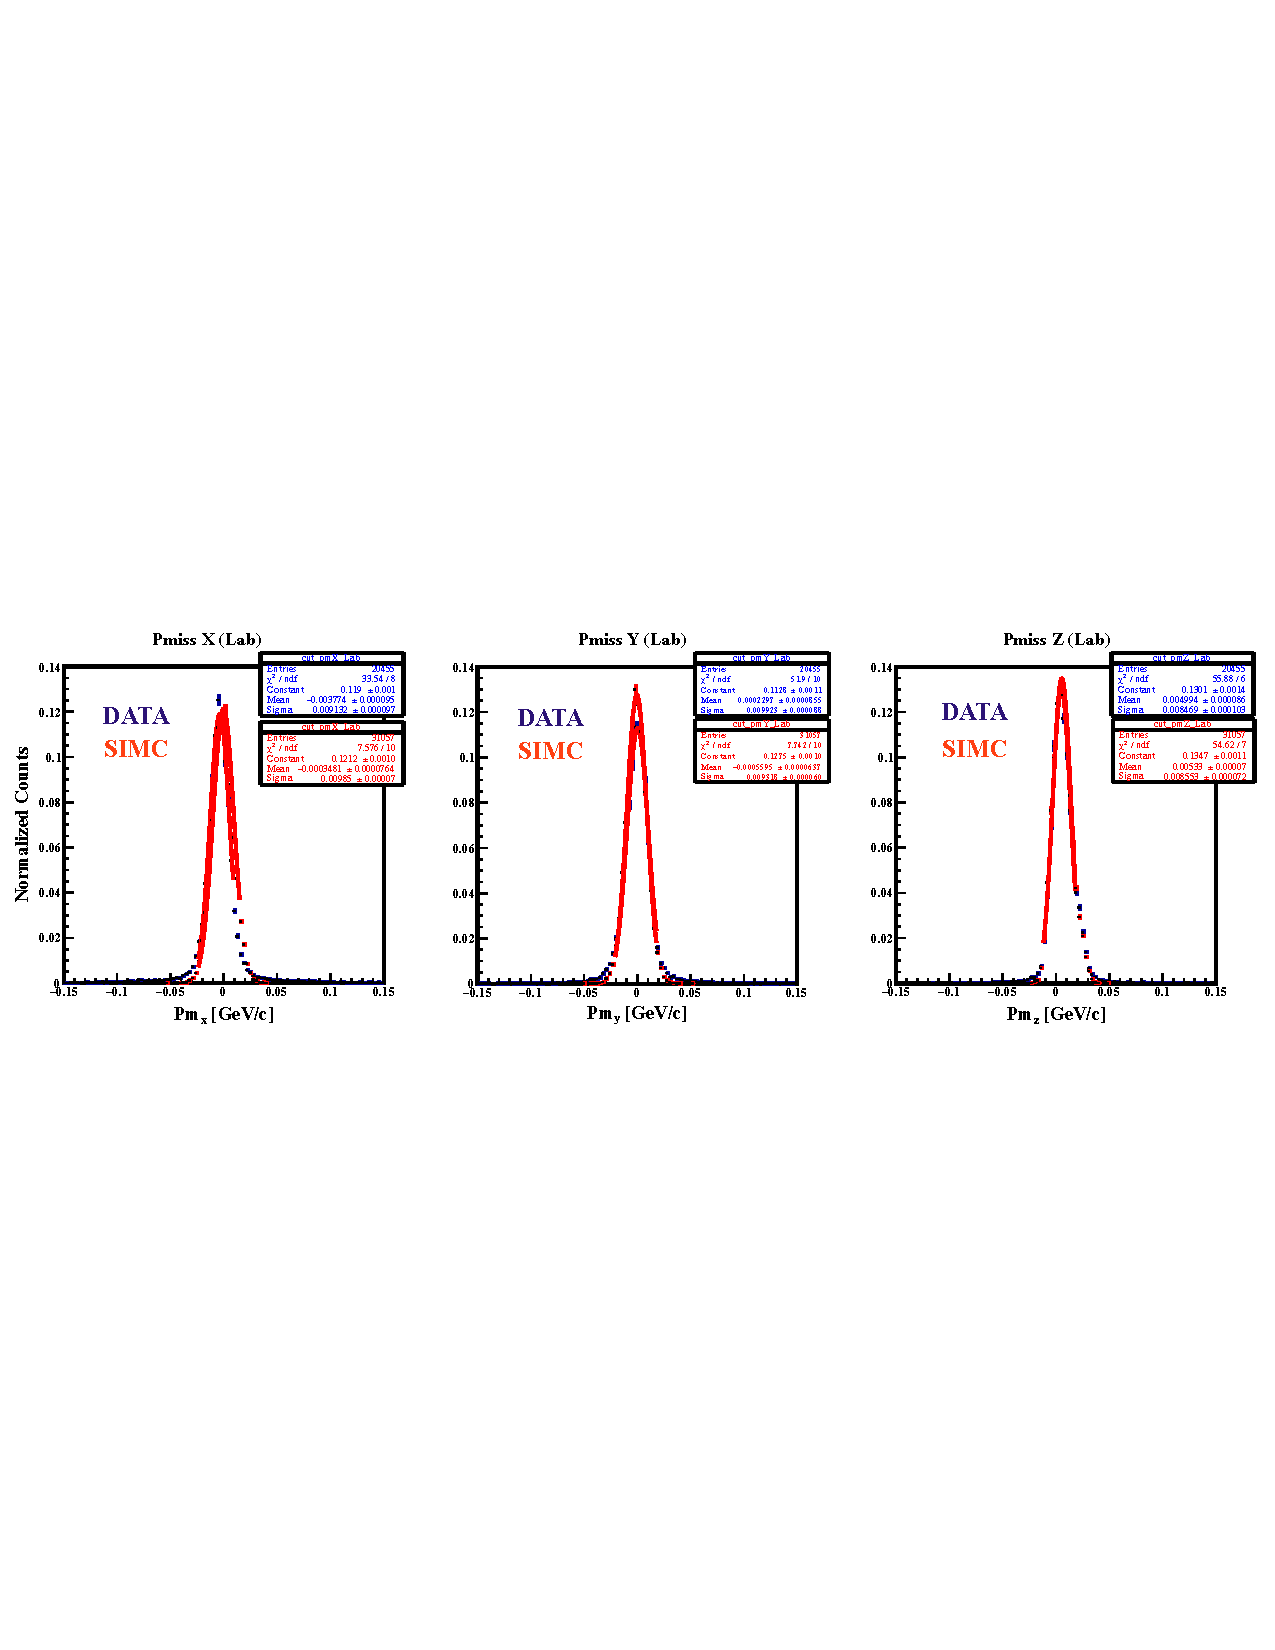
\includegraphics[scale=0.9]{plots/Oop_Pm_Offset.pdf}
  \caption{Missing Momentum components with Out-of-plane central offset applied.}
  \label{fig:PmComp_OopOffset}
\end{figure}\\

\noindent After applying the \textit{out-of-plane} offset, the Y-component of the missing momentum agrees with simulation as shown in Figure \ref{fig:PmComp_OopOffset}.
With respect to the X-component of the missing momentum, it was decided not to apply an \textit{in-plane} angle offset as
this would directly impact the location of the invariant mass peak. Alternatively, it was decided to apply a relative in-plane
angle offset which would align the X-component. This is discussed in the next sub-section.\\
\newpage
\subsection{Relative Angle Offsets}
The relative angle offsets refer to the angle offset relative to the spectrometer central ray. The two cases are:
\begin{itemize}
\item \textit{In-plane relative angle ($Y'_{tar}$) offset} \texttt{[h(p)theta\_offset]}
\item \textit{Out-of-plane relative angle ($X'_{tar}$) offset} \texttt{[h(p)phi\_offset]}
\end{itemize}
The $Y'_{tar}$ offset if directly related to the spectrometer angle, and therefore has a direct impact on the electron/hadron kinematics, depending on which
spectrometer is associated with the particle type. In the E12-10-003, this offset was determined for the HMS in order to align the X-component of the missing
momentum as well as to improved the HMS central momentum correction. Recall that in Section \ref{sec:hms_optics_sec} it was assumed that the proton (HMS) angle
was well known, which was not completely true. 
\begin{figure}[h!]
  \centering
  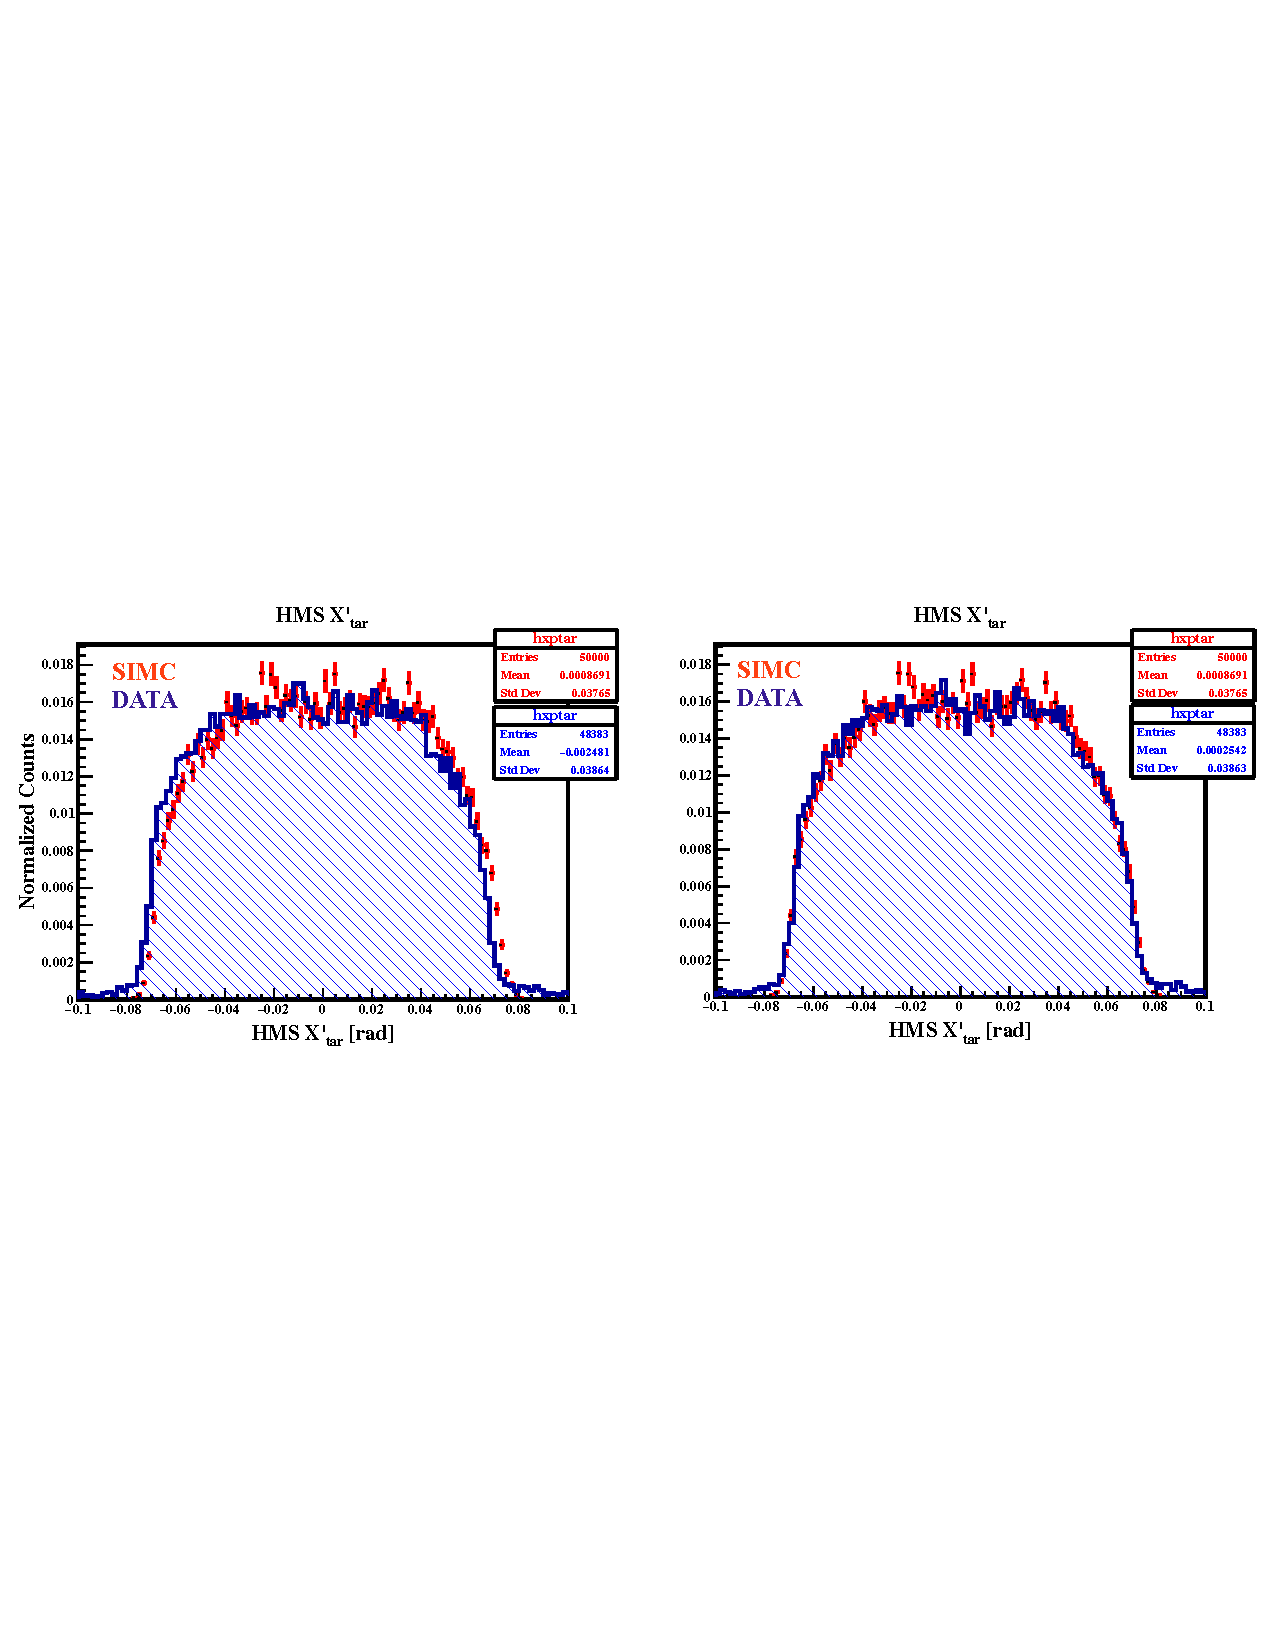
\includegraphics[scale=0.8]{plots/hxptar_offset_3288.pdf}
  \caption{HMS $X'_{tar}$ for run 3288 before (Left) and after (Right) applying the offset correction.}
  \label{fig:hxptar_Offset}
\end{figure} \\
Figure \ref{fig:hxptar_Offset} shows the relative out-of-plane angle distributions for all events within the spectrometer acceptance. The 'zero' value in the distribution
represents events whose trajectory was parallel to the central ray, whereas events away from the 'zero' value represents events that are at an out-of-plane angle relative
to the central ray. The $X'_{tar}$ offset was determined by 'eye', using the mean of the distribution. \\
\indent Similarly to the relative out-of-plane angle, the relative in-plane angles in the $Y'_{tar}$ distribution (not shown) represent angles relative to the central ray, with the
'zero' value representing particles parallel to the central ray. The $Y'_{tar}$ offset was determined based on how well the X-component of the missing momentum matched
the simulation, as well as how well did the HMS momentum from data matched that of simulation (See Figure \ref{fig:hms_Pcorr}). \\
\indent After determining the spectrometer offsets, a second iteration of the HMS and SHMS Optics check procedure was performed to obtain
improved results. Finally, the four H(e,e'p) elastic runs were used to determine the HMS momentum corrections for the D(e,e'p) data, to be discussed in the next section.
\section{HMS Momentum Calibration}
During the E12-10-003 experiment, the four H(e,e'p) elastics analyzed covered the HMS momentum range such that the D(e,e'p) data
momentum was within the range covered by the elastics. From this knowledge, one can determine the D(e,e'p) data momentum correction
from a simple linear fit of the H(e,e'p) data. 
\newpage
\begin{figure}[h!]
  \centering
  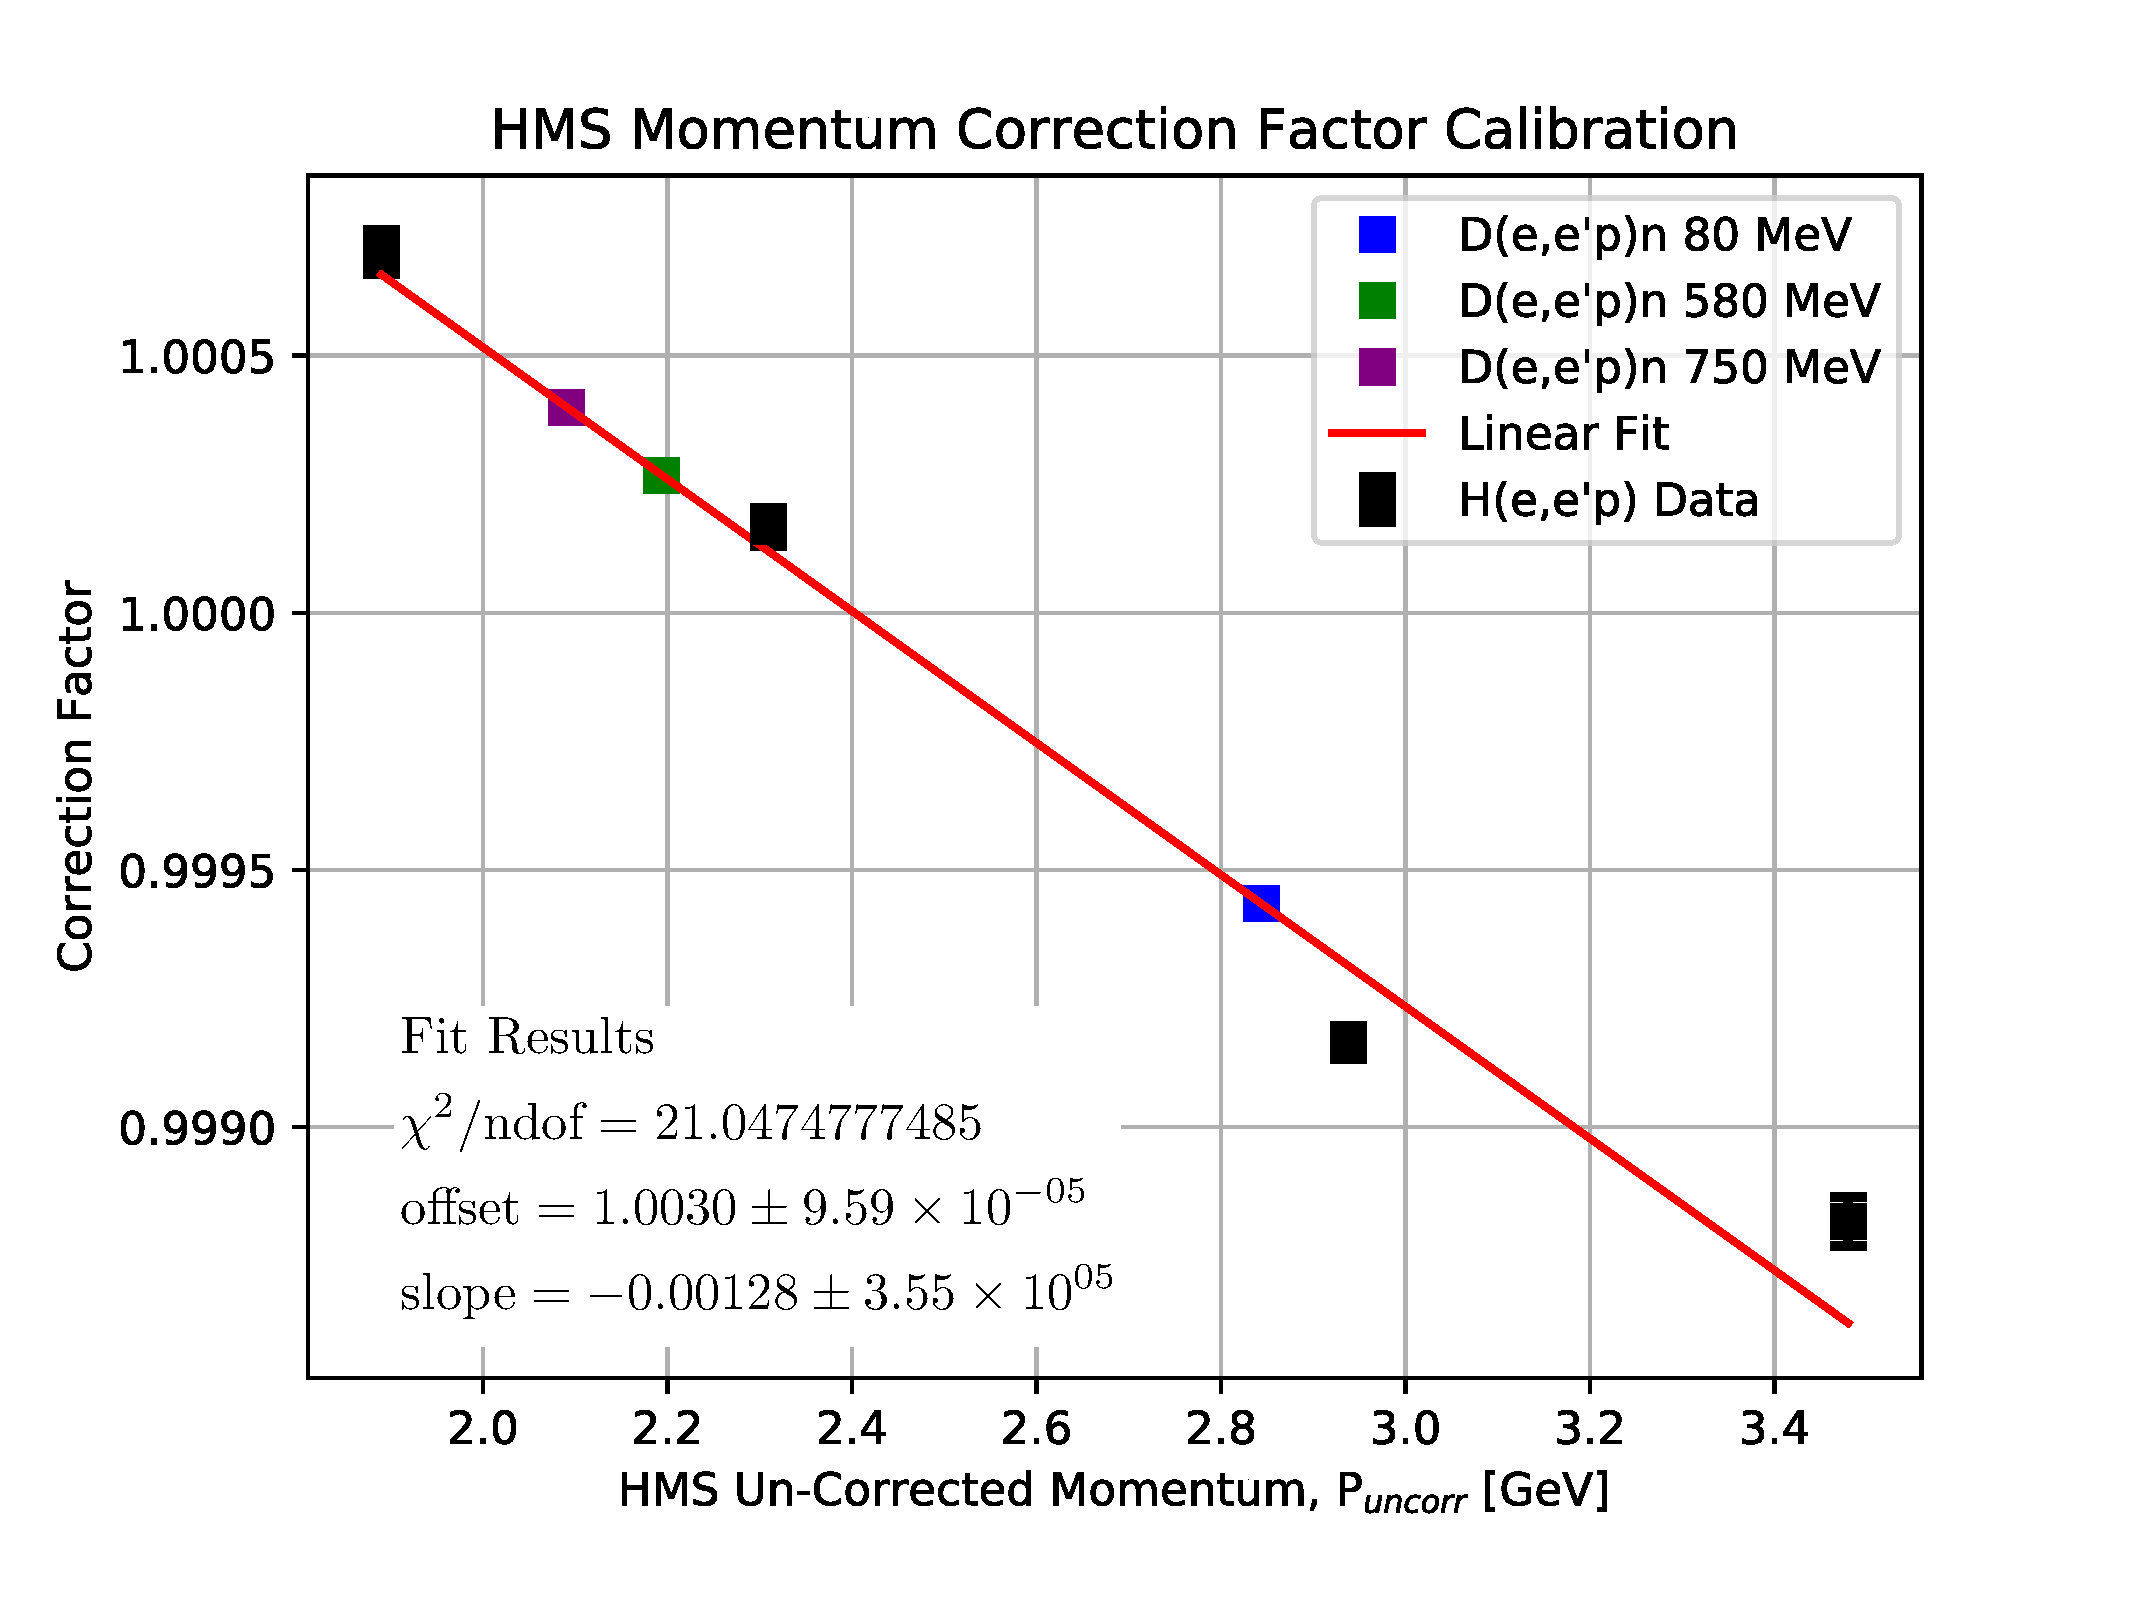
\includegraphics[scale=0.4]{plots/HMS_Pcorr_Fit.pdf}
  \caption{HMS Momentum Correction for H(e,e'p) and D(e,e'p)n. }
  \label{fig:hms_Pcorr}
\end{figure} 
\indent From Figure \ref{fig:hms_Pcorr}, the momentum correction factor is plotted against the original HMS central momentum and the
four data points are fitted with a straight line. Using the line fit, the D(e,e'p)n momentum correction for the three missing
momentum settings are determined from the D(e,e'p)n original HMS momentum setting. The table below summarizes the
correction to the D(e,e'p)n data HMS momentum settings.
\begin{table}[ht]
\begin{tabular}{c c c c c}
\hline\hline
\shortstack{$P_{m}$ \\ Setting [GeV]}  & \shortstack{HMS \\ Angle [deg]} & \shortstack{HMS \\ Momentum [GeV]} & \shortstack{SHMS \\ Angle [deg]} & \shortstack{SHMS \\ Momentum [GeV]} \\
\hline
80 & 38.896 & 2.8438 & 12.194 & 8.7 \\
580 (set1) & 54.992 & 2.194 & 12.194 & 8.7 \\
580 (set2) & 55.000 & 2.194 & 12.194 & 8.7 \\
750 (set1) & 58.391 & 2.091 & 12.194 & 8.7 \\
750 (set2) & 58.394 & 2.091 & 12.194 & 8.7 \\
750 (set3) & 58.391 & 2.091 & 12.210 & 8.7 \\
\hline
\end{tabular}
\label{table:original_deep_kin}
\caption{Original D(e,e'p)n Kinematics for E12-10-003.}
\end{table}
\begin{table}[h!]
\begin{tabular}{c c c c c}
\hline\hline
\shortstack{$P_{m}$ \\ Setting [GeV]}  & \shortstack{HMS \\ Angle [deg]} & \shortstack{HMS \\ Momentum [GeV]} & \shortstack{SHMS \\ Angle [deg]} & \shortstack{SHMS \\ Momentum [GeV]} \\
\hline
80 & 38.896 & 2.840 & 12.194 & 8.5342 \\
580 (set1) & 54.992 & 2.1925 & 12.194 & 8.5342 \\
580 (set2) & 55.000 & 2.1925 & 12.194 & 8.5342 \\
750 (set1) & 58.391 & 2.0915 & 12.194 & 8.5342 \\
750 (set2) & 58.394 & 2.0915 & 12.194 & 8.5342 \\
750 (set3) & 58.391 & 2.0915 & 12.210 & 8.5342 \\
\hline
\end{tabular}
\label{tab:corr_deep_kin}
\caption{Corrected D(e,e'p)n Kinematics for E12-10-003.}
\end{table}\\
The Table above shows the corrected HMS momentum for the deuteron kinematics. Since the SHMS momentum was un-changed during the experiment,
the single correction factor determined from the H(e,e')p data analysis applies for all runs. 
%Bibliography
\newpage
\onecolumn
\bibliography{d2_optim.bib}
\bibliographystyle{abbrv}

%APPENDIX
%\newpage
%\begin{appendices}
%\appendix
%\section{Appdx Section 1}
%\subsection{SubSection 1 . . .}
%\label{appendix:AppxA1}
%\end{appendices}

\end{document}
